% !TeX TXS-program:bibliography = txs:///biber
% $Id$
% Authors: Flavio Stancchi, Hautahi Kingi, Lars Vilhuber, Sylverie Herbert
% Results from the Cornell Replication Lab

%!Rnw weave = knitr
\documentclass[utf8]{article}
\usepackage{inputenc}

\usepackage[]{graphicx}\usepackage[]{xcolor}


\definecolor{shadecolor}{rgb}{.97, .97, .97}
\definecolor{messagecolor}{rgb}{0, 0, 0}
\definecolor{warningcolor}{rgb}{1, 0, 1}
\definecolor{errorcolor}{rgb}{1, 0, 0}

\usepackage{alltt}

% setting article items used multiple times
\newcommand{\mytitle}{Reproduce to Validate: a Comprehensive Study on the Reproducibility of Economics Research}
\newcommand{\myauthorA}{Hautahi Kingi}
\newcommand{\myauthorB}{Flavio Stanchi}
\newcommand{\myauthorC}{Lars Vilhuber}
\newcommand{\myauthorD}{Sylv\'erie Herbert}

% loading packages
\usepackage{lscape}
\usepackage{dcolumn}
\usepackage[printonlyused]{acronym}
\usepackage{pdfpages}
\usepackage{placeins}
\usepackage{amssymb}
\usepackage{amsfonts}
\usepackage{amsmath}
\usepackage[nohead]{geometry}
\usepackage[singlespacing]{setspace}
%\usepackage[bottom]{footmisc}
%\usepackage{indentfirst}
\usepackage{graphicx}
\usepackage{rotating}
%\usepackage[capposition=top]{floatrow}
\usepackage{float}
\usepackage{tikz}
\usetikzlibrary{calc}
%\usepackage{qtree}
\usepackage{makecell}
\renewcommand\theadalign{bl}
\usepackage{comment}
\usepackage{etoolbox}
\usepackage{csquotes}
%\usepackage{footnote}
%\makesavenoteenv{tabular}
%\makesavenoteenv{table}
%\usepackage{footmisc}


\usepackage{hyperref}
%\usepackage{biblatex}
\hypersetup{%
naturalnames=true,%
bookmarksnumbered=true,%
bookmarksopen=false,%
plainpages=false,%
colorlinks=true,%
linkcolor=black,%
citecolor=blue,%
urlcolor = black,
pdftitle={\mytitle},%
pdfpagemode=UseOutlines,%
pdfauthor={\myauthorD, \myauthorA, \myauthorB, \myauthorC},%
pdfsubject={Replication}
}
\usepackage{csvsimple}
\usepackage{xspace}
%==================== final toggle ====================%
%%%%%%% The "final" flag toggles the final version of the proposal. When set
%%%%%%% to true, all comments are hidden, the page is set to the correct size,
%%%%%%% and any `fix' information is drawn normally.
\newtoggle{final}
\toggletrue{final}
%\togglefalse{final}

%% Set margins for toggle
\iftoggle{final}{
    \geometry{letterpaper,left=1.0in,right=1.0in,top=1.0in,bottom=1.0in} %rgb
}{
    \geometry{letterpaper,ignoreheadfoot,left=1.0in,right=2.0in,top=1.0in,bottom=1.0in,footskip=0.25in,headsep=0.125in,marginparwidth=1.75in,paperwidth=9.5in} %rgb
}

%% enable todo package for margin notes, missing figs, and such
\iftoggle{final}{
        \usepackage[disable]{todonotes}
    }{
    \usepackage[textsize=scriptsize]{todonotes}
    }

% todo-enabled version: \margincomment{}{} command to put comments about text into the margin.
\newcommand{\mc}[2]{% % 1=initials, 2=comment
\todo[size=\scriptsize,linecolor=blue!90]{\textbf{\uppercase{#1}:}~#2}
}

%==================== bibliography tools

%\usepackage[backend=biber,sortlocale=nb_NO,sortcites,style=authoryear-icomp,doi=true,isbn=false,url=false,uniquename=false]{biblatex}
%\usepackage[backend=bibtex,style=authoryear,natbib,sortcites,doi=true,isbn=false,maxcitenames=2,date=year,url=false,eprint=false]{biblatex}
\usepackage[backend=biber,natbib,
%sortcites,
doi=true,isbn=false,maxcitenames=2,date=year,url=false,eprint=false,
authordate,ibidtracker=false]{biblatex-chicago}
%
\AtBeginRefsection{\GenRefcontextData{sorting=nyt}}
\AtEveryCite{\localrefcontext[sorting=ynt]}

\usepackage[american]{babel}
%\addbibresource{./includes/replication_papers.bib}
\addbibresource{./includes/paper.bib}
\addbibresource{./includes/aej-paper.bib}

%%%%%%%
\setcounter{MaxMatrixCols}{30}

%\makeatletter
%\def\@biblabel#1{\hspace*{-\labelsep}}
%\makeatother
%\geometry{left=1in,right=1in,top=1.00in,bottom=1.0in}
%\setlength{\parindent}{4em}
%\setlength{\parskip}{1em}
%%%%%%%%%%%
\setstretch{1.5}
\IfFileExists{upquote.sty}{\usepackage{upquote}}{}

\begin{document}





% NOTE: All R processing is done from the programs/ directory (README.Rmd) prior to running this file!
% The file config.tex contains the relevant paths

% Automatically created, do not edit
\newcommand{\TexIncludes}{/home/rstudio/text/includes}
\newcommand{\ROutputs}{/home/rstudio/text/analysis}
\newcommand{\Rprograms}{/home/rstudio/programs}


% possible overrides : relative paths
\renewcommand{\ROutputs}{analysis}

\title{\mytitle}
\author{\myauthorD\thanks{Banque de France: sylverie.herbert@banque-france.fr} \and \myauthorA\thanks{Google: hautahikingi@gmail.com} \and \myauthorB\thanks{Airbnb: fs379@cornell.edu} \and \myauthorC \thanks{Labor Dynamics Institute, Cornell University: lars.vilhuber@cornell.edu. This work has benefited from insightful comments by Christophe P\'erignon, Ben Greiner, Jan H\"offler, and participants of the Banque de France DGSEI seminar and the 2018 BITSS annual meeting at UC Berkeley. The paper has been previously circulated as \citet{kingi2018} and \citet{herbert2021}.  The opinions expressed in this article are solely the authors', and do not represent the views of the American Economic Association, the US Census Bureau, Banque de France, Google, or Airbnb. }}

\maketitle
% \begin{center}
% Preliminary - do not cite or quote without contacting authors.
% \end{center}
\sloppy

\begin{abstract}



\noindent
Journals have pushed for transparency of research through data availability policies. Such data policies improve  availability of data and code, but what is the impact on reproducibility? We present results from a large reproduction exercise for  articles published in the American Economic Journal: Applied Economics, which has had a data availability policy since its inception in  2009. 
%
Out of 363 published articles, we assessed  274 articles. All articles provided some materials. We excluded 122 articles that required confidential or proprietary data, or that required the replicator to otherwise obtain the data (44.5\% of assessed articles). 
%
We attempted to reproduce 152 articles, and were able to fully reproduce the results of 68  (44.7\% of attempted reproductions). A further 66 (43.4\% of attempted reproductions) were partially reproduced. Many articles required complex code changes even when at least partially reproduced. We collect bibliometric characteristics of authors, but find no  evidence for author  characteristics as determinants of reproducibility. There does not appear to be a citation bonus for reproducibility.

The data availability policy of this journal was effective to ensure availability of materials, but is insufficient to ensure reproduction without additional work by replicators. 


\end{abstract}

\textit{JEL} codes: B41; C80; C81; C87; C88

\setstretch{1.5}

\textbf{Keywords:} Replication, reproducibility, transparency, replicability, journal policies\\

%\singlespacing

\thispagestyle{empty}

\onehalfspacing
\clearpage

%%%%%%%%%%%%%%%%

\clearpage

% Note:
% Child documents:
%   if pure LaTeX,, use \include{document.tex}
%   if knitr document, use <<mypart, child='mypart.Rnw'>>==
%%
%%===================== Intro ======================
%%
\section{Introduction}\label{sec:intro}
Replication, reproduction, and falsification of published articles are important steps in the scientific process. These activities help to make science ``robust and reliable'' \parencite{Bollen2015-vb} and are a \textit{sine qua non} condition for the credibility of economic research. Robust and replicable research is especially important in policy institutions such as central banks or governments since it provides input needed for its core activities and informs their decisions. Given its importance for both research and policy purposes, the reproducibility and replicability\footnote{For precise definitions of these terms, see \parencite{Bollen2015-vb,nasem2019} and definitions in the next section.} of articles has been discussed in economics for at least thirty years\footnote{\textcite{Dewald1986,Vinod2005,AndersonEtAl2005,King95,BurmanEtAl2010,Duvendack2017,Hamermesh2017,Sukhtankar2017,Hoeffler2017,Coffman2017,Chang2017,Berry2017,Anderson2017}}. Since the early 2000s, many economics journals have a data availability policy requiring authors to deposit materials sufficient to reproduce the analysis in their article. The goal is twofold: the exercise of compiling the replication package itself provides an opportunity for authors to fix errors on their own. And the availability of these materials is meant to reduce the cost of replication and as a ``starting point for other researchers'' \citep{bernanke2004}. However, compliance is typically only lightly monitored (some authors have referred to it as the ``honors system''), and no pre-publication verification is conducted. In this paper, we carry out a large reproducibility exercise of published articles in a journal which implements such data availability policy.

Actual published reproductions or replications are rare \parencite{BellMiller2013b,Duvendack2017}, notwithstanding some recent examples \parencite{Hoeffler2017a,Chang2017,ChangLi2015,camerer2016}. For example, \textcite{MuellerLanger18} found that just 0.1\% of the 126,505 articles published between 1974 and 2014 in the top 50 economics journals were replications. \textcite{sukhtankar17} found that, of the 1,138 empirical development economics articles published between 2000 and 2015 in the ``top 10" economics journals,\footnote{\textcite{sukhtankar17} combines the traditional ``top 5" with the \ac{AEJ:AE}, the \ac{AEJ:EP}, the \ac{EJ}, the \ac{JEEA} and the \ac{ReStat}.} just 6.2\% were replicated in a published or working paper. The paucity of replications in economics is, in part, because it is often difficult to find the materials required to conduct reproducibility or replication exercises \parencite{Dewald1986,McCullough2006,McCullough03}. Despite a long standing explicit recognition of the importance of replication in economics \parencite{Frisch1933}, it has been suggested that ``there is no tradition of replication in economics" \parencite[p. 1093]{McCullough2006}.\footnote{Though \textcite{Hamermesh2007,Hamermesh2017} disagrees.} An exception has been the Journal of Applied Econometrics (since 2003) and more recently the newly created \ac{JPE} Micro, announced in February 2022.
 % This sentence may be too general. The scientific community is actively engaged in identifying ways to support replication \parencite{Bollen2015-vb,NAP25116}.}

To promote transparency, journals have adopted ``data (and code) availability'' policies (DAP). The \ac{AEA} announced one in 2004 \parencite{bernanke2004}, the \ac{JPE} in 2004, the \ac{QJE} was one of the last major economics journals to do so in 2016. Data availability policies require authors to make all data (and generally code) necessary to reproduce their study available, or when legal restriction prohibit the sharing of the data, authors should explain how to get access to the data. As of 2016, the top five economics journals all have a DAP. However, it is still not the norm among economics journals. Studies find that between 57\% and 66\% of economics journals (with some empirical content) have a DAP that requires or suggests deposit of materials, and between 12 and 14\% let authors provide materials on request \parencite{Hoeffler2017,vlaeminck2021}. There are also differences in the coerciveness of the DAP across journals, with only a small minority making deposit of materials mandatory\footnote{\textcite{Hoeffler2017}: in 2015, of 343 journals, 26 had mandatory DAP, 110 had voluntary DAP, and 49 allowed authors to provide data and code on request, possibly in combination with the offer of a deposit. \textcite{vlaeminck2021}: of 327 journals, 50 had a mandatory DAP, 135 had a voluntary DAP, and 38 had some sort of provision on request.}. Such DAP are not necessarily a panacea, as authors who have tested them in some way note it does not guarantee obtaining all the papers' codes and data, nor does it guarantee reproducibility \parencite{Glandon2010,Hoeffler2017,Stodden2018}.

More recently, journals and societies have appointed ``data editors'' responsible for monitoring compliance. The Canadian Economic Association appointed a data editor  in 2017. The \ac{AEA} appointed one of this article's authors as data editor in 2018  \parencite{10.1257/pandp.108.745} and subsequently updated its data and code availability policy. Similar positions have been created at the Review of Economic Studies, the Economic Journal, Management Science, and most recently, Econometrica. 
%According to  \textcite{Duvendack2015} only  27 of the 333 economics journals \mc{HK}{Should we update this?} listed in the Thomson Reuters \textit{Web of Science} as of September 2013 regularly publish data and code for empirical articles, and 10 of those journals explicitly state that they publish replication studies. While that number seems low, it is higher than it was a decade earlier. More recently, the \ac{JASA} has moved towards much more stringent replication requirements \parencite{Fuentes2016-wz}, and 

In this paper,  we set out to assess how well a particular journal's ``data availability'' policy, lightly monitored as described in the next section, yields \textit{reproducible} articles. We call the monitoring ``light'', because no verification of completeness or functionality was conducted prior to publication, in contrast to the more recent monitoring conducted by dedicated data editors. In other words, we ask the question: given that authors are required to provide code and data, without pre-publication verification, is that enough to generate reproducible results?


%
% Not relevant, because a very different exercise. Leave to conclusion.
% More recently, \textcite{perignon2022} analyze the reproducibility of more than 1,000 xxxfinance papersxxx (NOT PAPERS) through a controlled experiment. They task 168 research teams to answer six research questions using the same data. In our case, some papers might be assigned more than once, but it is the minority. We set to answer a slightly different question: 


Our protocol sets a relatively high bar: Can \textit{undergraduates}, armed only with the information provided by authors on the journal website, successfully reproduce the tables and figures presented by the author in the article? Unlike \textcite{Dewald1986} and \textcite{McCullough03}, who requested data and programs from the original authors, we did not attempt any contact with authors to clarify issues that arose. While our replicators were instructed to do their best to fix any bugs or inconsistencies that they encountered, they were limited both by time and training. On the other hand, it would seem that pure computational reproducibility should be the lowest standard met by an article.
We conducted this experiment over several summers starting in 2014 and during the 2018 fall semester, using the \ac{AEJ:AE} as our source of articles.

%
% parts moved to Background
%
We find a  moderate replication success, with a reproduction rate of 37.8$\%$ overall. 44.7$\%$ of articles were successfully reproduced, conditional on  data being available, with an additional 43.4$\%$ partially reproduced. Compared  to a reproduction rate of $13\%$ found by \textcite{Dewald1986} in the context of a journal (\ac{JMCB}) with no data or code availability policy, our results seem to suggest that journal policies that enhance transparency are helpful, yet not sufficient to reach full reproducibility. We further show that fully reproducible papers do not seem to benefit from a citation bonus ---  authors' reputation seems to matter the most when it comes to citations. We speculate that we mafy be in a relatively low reproducibility equilibrium because the costs of producing reproducible research (for instance in terms of time) outweigh the advantages (given it does not lead to more citations). Our contribution to the literature is thus twofold: (1) we provide an estimate of reproducibility standards of a journal that imposed, since its founding, a data availability policy; (2) we provide a rationale for authors' lack of incentives to produce reproducible research, absent journals' verification of reproducibility.


%%The tools for successful reproduction studies (which henceforth we will use to designate basic validation studies and robustness or perturbation checks) have become more widely available in recent decades,
%Short of tackling the thorny issue of how to publish replication studies, journals have attempted to provide forums for discussions of the robustness of published results.  For instance, \url{arxiv.org} and the American Economic Association have made available comment sections for any article published, so that focused scientific discussion could be made in a public forum. Unfortunately, adoption of these tools is rather weak. A scan of several years of American Economic Journals shows very little use:
%% 2014-10-09
%% awk -F, ' { sum+=$2; n+=1 } END { print sum,n } ' *csv
%% awk -F, ' { print $2 } ' *csv | sort
%out of 254 articles in the \textit{American Economic Journal: Applied Economics} (as of October 2014, and since inception), a total of 19 comments had been posted on 14 articles (the largest count was 3, and those all came from the author of the paper itself!).
%%
%One possible conclusion is that comment sections don't give the appropriate academic rewards (citability) that journal articles or similar venues would provide.
%Even when discussion does occur in other (less formal) forums, it can often become acrimonious, which can discourage both junior and senior academics from participating.




%\mc{HK}{Lars, this paragraph might be too speculative/irelevant. It's just my attempt to explain which part of the replication crisis our work best addresses. Delete if necessary.} \textcite{Christensen2018} identify several problems with the current scientific enterprise that help to explain the failure of many research findings to replicate - from researcher fraud and publication bias to simple sampling variation. Our focus on a narrow or minimal sense of reproducibility addresses most directly the issue of ``specification searching" \parencite{Leamer1983,Lalonde1986} or ``the garden of forking paths" \parencite{Gelman2013}, in which researchers make numerous analytical decisions in the process of, say, data cleaning or model selection, to arrive at an ``interesting" result, either consciously or unconsciously. The presence of computer programs that reliably reproduce the reported results can help to make explicit these various decisions taken during the research process, and help to explain why independent replications, which inevitably make different decisions, fail.

%In this article,  we set out to assess how well a particular journal's ``data availability'' policy, combined with light enforcement, yields reproducible articles. All articles stem from a small selection of \ac{AEA} journals, so we can therefore begin to assess cross-journal variation in enforcement or details of such policies. Our protocol is set with a relatively high bar: can undergraduates, armed only with the information provided by authors on the journal website, successfully reproduce the tables and figures presented by the author in the article? Unlike \textcite{Dewald1986} and \textcite{McCullough03}, who requested data and programs from the original authors, we did not attempt any contact with authors to clarify any issues that arise, and while  our replicators are instructed to do their best to fix any bugs or inconsistencies that they encounter, they are limited both by time and training.

%
%\footnote{The choice of years is quite arbitrary. We started with the 2013 volume in the summer of 2014, then added two additional, earlier years in the summer of 2015, to better capture post-publication outcomes such as citations.}
%

%We conducted this experiment over several summers and during the 2018 Fall semester, using four journals produced by the \ac{AEA}. For the first three summers from 2014-2016, we focussed soldely on the \ac{AEJ:AE} as our source of articles. We chose the \ac{AEJ:AE} primarily for two reasons. First, because of the empirical nature of its articles and its policy of publishing papers ``only if the data used in the analysis are clearly and precisely documented and are readily available to any researcher for purposes of replication," we expect that nearly all articles have some empirical component. Second, while other journals may also have theoretical or more complex empirical papers, using a variety of software, we wanted articles to be reproducible by the undergraduate student armed with knowledge of Stata and Matlab only. However, nothing in the methodology used in this paper was specific to the \ac{AEJ:AE}, and we later expanded our sample of articles to the \ac{AEJ:Mic}, the \ac{AEJ:Mac} and the \ac{AER}. Part of the motivation here is also to test the feasibility of ``pre-publication verification'' similar to what is done at the \ac{AJPS} \parencite{JacobyShouldJournalsBe2017,Christian2018}



We start by describing, in Section~\ref{sec:methodology}, our methods of selection, analysis, and reproduction. We present our results in Section~\ref{sec:results} before concluding in Section~\ref{sec:discussion}.

%

%%
%%===================== Background ===================

\section{Background}\label{sec:background}
% Background
% 
% in part in response to Ref 1, Q2 
%
The focus of the exercise is to assess whether availability of replication packages, in compliance with a posted data availability policy, leads to reproducibility. It is thus worthwhile to briefly discuss the policy as it was applied at AEA journals. 

The policy was first announced by \citet{bernanke2004}. Authors would provide ``in electronic form, data and code sufficient to permit replication [sic].'' It is unknown when the policy was separately posted on the AEA's website, but the policy as of 2018  \citep{American_Economic_Association2008-wayback} is largely consistent with the original (very brief) statement. Authors would email (or upload to an FTP server) ``data set(s) and programs used to run the final models'', including a Readme PDF with instructions. Exemptions for ``proprietary'' data needed to be approved by the journal's editor. The American Economic Journals launched in 2009, and applied this policy from the outset. Exemptions are (at least in later years, and through 2020) tabulated in the annual editors' reports \citep[see f.i.][]{mas2019}.\footnote{We briefly touch on assessed reasons for exemptions in Section~\ref{sec:results}.} 

We chose the \ac{AEJ:AE}  for two reasons. First, because of the empirical nature of its articles and its policy of publishing papers ``only if the data used in the analysis are clearly and precisely documented and are readily available to any researcher for purposes of replication" \citep{American_Economic_Association2008-wayback}. As we outline in Section~\ref{sec:methodology}, we wanted replication materials to be present for all articles in the journal, without needing to contact authors. The \ac{AEJ:AE} applied the AER's data availability policy from its creation in 2009. From past experience of this team \citep{vilhuber2020a} and others \citep[e.g.][]{Dewald1986,McCullough03,Stodden2018}, requesting materials from authors is fraught with non-response. 

%we expect that nearly all articles have some empirical component.
The second reason for the choice of the \ac{AEJ:AE} was based on feasibility. A cursory review of the articles on the \ac{AEJ:AE} website suggested that articles would be less complex than articles in the \ac{AER} or Econometrica, including by using mostly high-level software commonly used in economics, such as Stata and MATLAB.%
%
\footnote{See \citet{VilhuberAEAPap.Proc.2020} for a distribution of software used in replication packages deposited by authors in AEA journals from 1999 to 2018.}
% while other journals may also have theoretical or more complex empirical papers, using a variety of software, 
We wanted articles to be reproducible by undergraduate, students who are mostly armed with knowledge of Stata and MATLAB.%
%
\footnote{In practice, all articles in \ac{AEJ:AE} use Stata for most of the analysis, but some use additional softwares. We address this in Section~\ref{sec:results} in more details.}
However, nothing in the methodology used in this paper is specific to the \ac{AEJ:AE}, and could be applied to other journals. 

An additional, though not crucial, motivation, was to test the feasibility of ``pre-publication verification'' at AEA journals, similar to what was, at the time, done at the \ac{AJPS} \parencite{JacobyShouldJournalsBe2017,Christian2018}. The results obtained from the exercise reported in this article ultimately lead to the implementation of pre-publication verification at the \ac{AEA} journals \parencite{10.1257/pandp.109.718,vilhuber2022a}.

The exercise reported here differs somewhat from many other articles in the space of reproducibility and replicability. Some author teams have attempted to replicate, rather than computationally reproduce, published articles, in particular in the field of behavioral economics and psychology \citep{opensciencecollaboration2015b,camerer2016,camerer2018}. Others have taken a less structured approach to computational reproducibility, by simply attempting to run any code within a replication package and check for failure \citep{trisovic2021,wang2020}. Finally, others have conducted replication exercises that were designed to identify cross-researcher degrees of freedom \citep{menkveld2023,huntington-klein2021}.



How does our exercise compare with and differ from similar exercises conducted in the past? 
\textcite{Dewald1986} attempted to reproduce 54 articles from the \ac{JMCB}, a few years after \ac{JMCB} had introduced a pioneering DAP. The policy was so pioneering that many authors did not comply: Only 49 out of 65 (75\%) provided replication materials to the journal upon request, despite the policy requiring it. They report a reproduction rate of  7 out of 54 (13\%) articles, though they only attempted to actually compute the results for nine articles, absent complete data and code for others (7 out of 9, 78\%). Only two were perfectly reproduced (either 2 out of 54, or 2 out of 9). In later work using the same journal, \textcite{McCullough2006} found only 14 of 196 (7.1\%) articles selected from the \ac{JMCB} that should have had archives were actually reproducible. Only 69 articles actually had replication archives, some of which were incomplete. Conditional on having code and data, they therefore succeeded in fully reproducing 14 out of 62 (22.6\%), though they did not have sufficient computational resources to test the reproducibility of seven others.

%2 Our paper studies the effectiveness of a DAP based on archives through a rigorous and large-scale reproducibility exercise.
This paper is not the first assessment of the AEA's DAP. In 2008, six PhD students attempted to reproduce 39 empirical articles out of 135  papers published in the AER between 2006 and 2008 \parencite{Glandon2010}. Out of 39 articles, 11 were based on proprietary data and only 9 papers were actually assessed for reproducibility. However, they also assessed completeness of the provided packages, and estimated that 95\% would be reproducible without help from the authors if data were accessible. By the replicators' assessment, none were perfectly reproducible, but more than half (five out of nine) had enough information that substantial effort to fill in the blanks would yield a perfect replication. The other four had immaterial discrepancies between the results and the published paper. 

\textcite{ChangLi2015}, using slightly different methodology in selection, selected all articles from 13 well-regarded economics journals, including the AER, satisfying certain criteria (empirical paper using data on U.S. gross domestic product), and successfully reproduced the results of only 22 of 67 papers (32.8\%). This seems to suggest that journal policies to enhance publications are helpful, but insufficient to foster reproducibility. Most closely related may be \textcite{greiner2023}, who enrolled 700 (unpaid) replicators for nearly 500 articles previously published in \textit{Management Science}, both before and after the implementation of a data and code availability policy. Conditional on having data, code, and IT infrastructure in place, they were able to reproduce 95\% of articles after implementation of the policy. They find that introduction of the data and code availability policy both increased availability and quality of replication packages. 


In a related exercise, \citet{Stodden2018} used articles, including in economics, published in \textit{Science} as the basis of their analysis. Given Science's policy, they had to request data for 180 (88\%) of the articles in their sample by contacting authors.  They only managed to obtain data and code for 89 (43.6\%) of their sample, and assessed 56 of these. In the end, they only attempted reproduction of 22 (10.8\%), for which 95\% were reproducible. 

A similar exercise, albeit not focused on published articles, is \citet{perignon2022}. In their case, they were able to re-purpose the 163 replication packages generated by the \citet{menkveld2023} project, and assess reproducibility of the code used to produce the 6 research questions of that project. It is a much narrower exercise, as all researchers who participated came from a small subfield of finance, and accomplished the programming task within a much more limited timeframe than the typical economics paper. At the same time, it is also more complex, as the choice of software varied more widely within this narrowly focused field than in the entire \ac{AEJ:AE} corpus, which had to be mastered by a single replicator. The lack of field diversity, topics, and replicator skill diversity allow a clean focus on the researcher skills leading to lack of reproducibility, something which in our context will be somewhat obscured by the intersection of researcher programming skills and replicator execution skills.


%%===================== Methods ======================
%%
\section{Methodology}\label{sec:methodology}

%% \section{Description of Reproduction Procedure}\label{sec:methodology}


We start by defining  terms and concepts, describing the setup for the reproducibility exercise, followed by the bibliometric analysis.
%
As in any modern study on ``reproducibility'' and ``replicability,'' we need to define those terms, since historically, multiple, often conflicting or confusing definitions have been used \parencite{Pesaran2003,Hamermesh2007,Bollen2015-vb,Clemens2015,nasem2019}
%
Throughout the text, we use (computational) \textit{reproducibility} to refer to ``the ability [$\dots$] to duplicate the results of a prior study using the same materials and procedures as were used by the original investigator'' (\citet{Bollen2015-vb}, see also \citet{nasem2019}). \textcite[p. 942]{Christensen2018} argue that is the ``basic standard [that] should be expected of all published economics research, and hope this expectation is universal among researchers.'' In contrast, \textit{replicability} refers to ``the ability of a researcher to duplicate the results of a prior study if the same procedures are followed but new data are collected.''%
%
\footnote{\label{fn:confusion}We note that we have ourselves not always been consistent in the use of these terms. For instance, our instructions to our ``replicators'' ask whether the article has been ``replicated'', not ``reproduced,'' see Appendix~\ref{app:assessment_form} and~\ref{app:exit_form}. While \citet{Bollen2015-vb} certainly first defined the concepts as we use them here, they only became (relatively well) accepted with the publication of \citet{nasem2019}, after the conclusion of our experiment. We reproduce our replicator instructions material verbatim in the appendix, and do not modify the terminology.}
%sec:
%and \textit{generalizability} refers to the extension of the scientific findings to other populations, contexts, and time frames, perhaps using different methods. Because there is a grey zone between these last two definitions, we will generally refer to either context as ``replicability'', which \textcite{Hamermesh2017} calls ``scientific replication.''} %Robustness tests performed by researchers have aspects of self-replication, by identifying conditions under which the findings continue to hold when software or data are varied.

%We will use these terms as defined, even when authors use different terms.
%In this text, we will use the terms as defined above when the distinction is material. However, we may refer to the overall concept of redoing the analysis as ``replicability''.}. In simple words, the same code and data should produce similar results. 
We refer to the collection of instructions, code, and data as ``replication packages,'' because they enable not just the exact computational reproduction of an article, but also more generally replication.%
%
\footnote{Journals sometimes do refer to these as ``supplemental data,'' but in economics, they almost always contains code, if not data.}
%
In our context, we will refer to the (junior) researchers re-executing the code in a replication package as ``replicators,'' primarily for linguistic convenience (see also footnote~\ref{fn:confusion}).

%
% Exercise setup
%
 
Our reproducibility exercise was conducted over the course of five summers, from 2014 to 2018 as well as the fall semester of 2018. The exercise was split into three steps.  
%
First, an ``assessor'' evaluated an article and its replication package as to the availability of the required components and its difficulty, and recorded a selection of article characteristics. A ``replicator'' then conducted the actual reproducibility check. Often but not always, the same person would be assessor and replicator. Finally, upon completion of the attempt at reproduction, replicators filled out a guided report with questions about the reproduction, such as whether or not the main results of the article could be reproduced and, if not, the main barriers impeding a successful reproduction. 

To complement the information collected during the reproducibility exercise, we also obtained descriptive article and author information, such as citations and h-indexes, from 
%Web of Science \parencite{WebofScience} and 
the OpenAlex (OA) \ac{API} \parencite{openalex2022,ourresearch2023}.

\subsection{Article selection}

The \ac{AEJ:AE} published 363 articles between the first issue in 2009 (volume 1 issue 1) and the April issue in 2018 (volume 10 issue 2). Replicators worked on this project from the summer of 2014 until Fall of 2018. Articles were added to the assignment set in groups by year, though somewhat haphazardly. The pilot project in the summer of 2014 worked on articles from 2013, and completed many of them. Subsequently, the collection of information was systematized, but the articles already completed from 2013 were not transferred to the new collection instrument, and are thus missing from our analysis in this paper. In 2015, using the systematized collection instrument,  years 2010 and 2011 were added. Years 2009 and 2012 were added in the summer of 2016, and publication year 2014 was added in 2017. Finally, in 2018, the years 2015 through 2017 as well as the first two issues in 2018 were added (see Appendix Table \ref{tab:assignments}). Articles were added in batches to separate online spreadsheets, based on a pull from the CrossRef API, which yielded articles in somewhat random order, augmented by a manual culling of unprocessed articles from the previous summer's list.%
%
\footnote{Ex-post inspection of our assignment lists shows no particular pattern, though articles with lower issue and page numbers seem to appear higher in the original lists.}
% 
Once a particular cohort of replicators had completed a batch, a new batch was pulled. 
%
Replicators were assigned an initial article by the supervising team, but could subsequently self-select (first come, first serve) from the list of unprocessed articles. They were instructed to finish the initial assessment regardless of the outcome. We do not believe that there was intentional systematic assignment based on data availability, software usage, or topic.


Table~\ref{tab:Selection} shows the number of eligible articles (i.e., published articles) per year, and the number of articles each year that were assessed and scored, as described in the next few sections. 


% Table created by stargazer v.5.2.3 by Marek Hlavac, Social Policy Institute. E-mail: marek.hlavac at gmail.com
% Date and time: Mon, Mar 11, 2024 - 12:57:41 AM
\begin{table}[!htbp] \centering 
  \caption{Articles Published and Selected by Year} 
  \label{tab:Selection} 
\footnotesize 
\begin{tabular}{@{\extracolsep{0.4pt}} cccccccccccc} 
\\[-1.8ex]\hline 
\hline \\[-1.8ex] 
  & 2009 & 2010 & 2011 & 2012 & 2013 & 2014 & 2015 & 2016 & 2017 & 2018 & Total \\ 
\hline \\[-1.8ex] 
Published & 34 & 40 & 37 & 40 & 38 & 40 & 35 & 37 & 42 & 20 & 363 \\ 
Selected & 21 & 23 & 32 & 39 & 8 & 40 & 21 & 33 & 39 & 18 & 274 \\ 
Percent & 61.76 & 57.5 & 86.49 & 97.5 & 21.05 & 100 & 60 & 89.19 & 92.86 & 90 & 75.48 \\ 
\hline \\[-1.8ex] 
\multicolumn{12}{l}{Notes: Assessments made using the entry questionnaire by replicators,} \\ 
\multicolumn{12}{l}{prior to attempting to reproduce any tables or figures. The sample of assessed} \\ 
\multicolumn{12}{l}{papers comprises those for which we had complete assessment questionnaires.} \\ 
\end{tabular} 
\end{table} 


\subsection{Initial Assessment}\label{sec:entry}

Before attempting a reproduction, each article was assessed.
%The replication process began with an ``Entry Questionnaire," which was filled out by an assessor before the replication
An assessor filled out the entry questionnaire, gathering descriptive information,  and providing an initial assessment of the expected level of reproducibility of an article.%
%
\footnote{See Appendix~\ref{app:assessment_form}. We will refer to questions on the entry questionnaire by ``Entry Q1'', ``Entry Q2'', etc.}
%
Each assessor was provided the  \ac{DOI} of the article,%
%
\footnote{\acp{DOI} are a managed identifier space built on top of the Handle System \parencite{Handle}, a technology for distributed, persistent, and unique naming for digital objects. Virtually all academic publishers assign \acp{DOI} at the article level in all of their publications. In addition, \acp{DOI} are increasingly used to identify data \parencite{PollardWilkinson2010}. In particular, each \ac{DOI} provides a persistent identifier \parencite{DOI2012} for a digital object: an article or data artifact.}
%
and then verified the following elements:
\begin{itemize}
\item
The presence of one or more downloadable datasets (including \ac{DOI} or URL, if any), an online appendix, the programs used by the authors and documentation on how to run them (the ``Readme");%
%
 \footnote{In theory, the author might have provided a \ac{DOI} to a third-party data archive for some or all of the content. 
 	%Ideally, each component -- the article, the online appendix, the data and the programs -- would have a separate \ac{DOI}. 
 	In the case of the \ac{AEJ:AE}, at the time this exercise was conducted, only the article itself was assigned a \ac{DOI}. Supplemental data, programs, and online appendices are linked from the landing page associated with the article's \ac{DOI}. This has changed since completion of the exercise, see \textcite{VilhuberAEAPap.Proc.2020}.}
 %
 \item
 The clarity and completeness of the documentation and of the program metadata;
 \item
 The presence of clear references to the original data provenance and a description of how to construct the initial datasets;
 %\mc{HK}{It doesn't look like we actually report anything about this information, and it was left blank for the majority of articles. Shall we just say that most articles didn't provide data provenance?}
 \item
 Data availability, and some basic categories if not available as part of the replication package (e.g., restricted access data, private data, public use data, etc.)
 \end{itemize}

%Although some of the responses to the questionnaire could have been captured via web-scraping tools, it is not possible to assess the completeness of the replication package without inspection by the assessor. 
While many supplemental data packages contained some content, they often did not contain all the data or programs. Sometimes, the data provenance might be described in an online appendix, while the instructions for the programs might be enclosed in the supplemental ``data'' package. Thus, a ``clerical'' review of each article's webpage, and some careful reading of the actual article and online appendix were the only way to collect all the information requested. 
%We will return to the aspect of machine-readability (machine-reproducibility) in the concluding discussion.

Based on the initial objective enumeration of the characteristics of the article and a subjective evaluation by the assessor of the complexity of the task described in the ``Readme" document, the assessor was asked to provide a subjective rating of the replication difficulty, from 1 (easiest) to 5 (most difficult), based on a set of heuristics (see Table~\ref{tab:criteria_difficulty}, Entry Q60).%
\footnote{A score of 1 assigned to an article does not imply that its replication package cannot be improved. For example, the programs provided by authors might lack documentation, or the provenance of the included datasets might be obfuscated, despite  the article being easily reproducible.}
Assessors also recorded the programming languages (Entry Q8) and separately the data storage formats (Entry Q21, Q28, Q36, Q44) contained within each archive. Archives can and do contain programs and data in multiple formats.
While all articles had some supplementary data, not all articles were accompanied by the datasets necessary for replication. Assessors recorded  whether the articles were accompanied by any data (Entry Q14), and if not, the (apparent) reason why data were not provided (Entry Q15). This included an assessment of whether the data were confidential or proprietary, for which we provided some guidance.


\begin{table}[!htbp] \centering
  \caption{Criteria for Assessment of Difficulty of Replication}
  \label{tab:criteria_difficulty}
\footnotesize
\begin{tabular}{@{\extracolsep{3pt}} cc}
\\[-1.8ex]\hline
\hline \\[-1.8ex]
Rating & Description   \\
\hline \\[-1.8ex]
\thead[bc]{~\\1\\~} & \thead{The article possesses all desired features that ensure replicability. Datasets are provided\\
and their use is public. The documentation and program metadata are clear and complete.\\ Negligible changes might be required to run the programs (e.g. path redirection).}\\
\thead[bc]{~\\2\\~} &  \thead{The article possesses most desired features that ensure replicability. Datasets are \\ provided and their use is public. The documentation and program metadata are present\\ but the programs might need some changes to run cleanly.} \\
\thead[bc]{~\\3\\~}  & \thead{The article replication may present some difficulties. Datasets are provided and their use\\ is public, but the documentation is incomplete or unclear. Substantial changes might be\\ needed to run the programs.}  \\
\thead[bc]{~\\4\\~} & \thead{The article replication may present substantial difficulties and/or additional steps are\\ required to recover the datasets used by the authors. Datasets may not be provided but\\ their use is public or available on request.}\\
\thead[bc]{5\\~} & \thead{The article is not replicable. The dataset are not provided and their access is private or\\ restricted. The programs are not provided. Documentation is absent or incomprehensible.}   \\
\hline \\[-1.8ex]
\end{tabular}
\begin{minipage}{0.8\textwidth}
NOTE: The description is reproduced verbatim. The language used in the instructions used ``replication'' instead of ``reproduction'', as we generally use it in this article.

\end{minipage}
\end{table}


\FloatBarrier



\subsection{Reproducing the Empirical Analyses}

Once the article was assessed and determined to be amenable for replication, a replicator was assigned based on characteristics of the article, and in particular the type of software required and the assessed difficulty of the replication task. Most often, the initial assessor self-assigned themselves as the replicator although some replications were conducted by the supervising team or distributed to a replicator based on their familiarity with a particular programming language.
%\footnote{The team used a restricted-access Subversion repository. }
The materials for each article were downloaded, and used to populate an article-specific repository. 
%
% Moved here
%
Unlike  \textcite{Dewald1986,McCullough03,Stodden2018}, who requested data and programs from the original authors when no materials were published by the journal, but similar to \textcite{Glandon2010}, we only tried to obtain data that was available on the journal's archive, and replicators were explicitly instructed not to contact the authors. This is very much in the spirit of \textcite{King95,McCullough2006,Glandon2010} and others, who emphasize the importance of being able to reproduce the results without assistance from the authors. Thus, we did not follow-up on  missing datasets, private data, protected data, or data available upon request. All attempts at reproducing the analysis were done based exclusively on the materials provided by the authors at the time of publication of the articles, or references therein leading to external data archives.
%If multiple replicators worked on the same article, they would work in separate subdirectories of the same repository.
%

The replicator was instructed to document any changes made to the author-provided programs using a \ac{VCS}. They also recorded information in two additional files: Any URLs that were used to download materials were recorded in \textit{`SRC.txt'}, and a high-level summary of steps undertaken for the replication and results obtained in a short report (called \textit{`REPLICATION.txt'}).

Once the \ac{VCS}  was populated and all data files  downloaded, each replicator was instructed to  read the author-provided ``Readme'', and attempt to run the programs in the author-provided archive. Replicators were told to keep modifications to the absolute minimum, starting with the adjustment of path structures to the replication system (for an example, see Appendix Figure~\ref{fig:svndiff}). Whenever a program required more extensive changes to run, the replicator would do so to the best of their ability. 
The entire team discussed problems encountered in regular meetings, and sought to find solutions. However, we also limited the time to find a solution for problems encountered to about a week. If unsuccessful in finding a solution, the reproduction attempt was marked as ``not reproducible.'' There was no time limit for running programs.

Replicators were free to use any computer they had access to for the replication, unless the author materials specifically mandated a particular operating system. This was quite rare, but did happen a few times. We note that the journal does not require authors to specify the required software, \ac{OS}, and versions thereof, and most articles were silent on the topic. In addition to replicators' laptops, our team had access to university-provided Windows remote desktops and a Linux cluster, and were unlikely to be constrained by computing resources. Both Windows and Linux systems had access to the latest version of the computing software, typically updated yearly.
% (%
% per correspondence with Janet Heslop, Director of IT, CISER, 2016-01-27
% at the time of the reproducibility exercise, Stata 13 and 14, the most current version of MATLAB, SAS 9.4, SPSS 23, and a recent version of Excel). 
%
In general, we assume that versions of \ac{OS} and software are different from the version originally used by the authors, given the considerable time lag between submission, publication, and the time of the reproducibility exercise. In some cases, programs needed small modifications to run cleanly due to software version discrepancies. If successful, these modifications were treated as `negligible' and did not affect the score of the article. If unsuccessful, however, the article was classified as non- or partially reproducible. We discuss the necessary code changes required for successful reproduction along with our results in Section~\ref{sec:results}.
%\footnote{We captured the modified programs created by the replicators in the \ac{VCS}. We could, therefore,  capture objective measures of code changes using, for instance, the number of code lines changed. However, this turned out to be more complex than expected, and was skipped for the analysis reported here.}


% MOVED TO CONCLUSION

%One way to address the issue of software versioning and other issues such as ambiguity in the documentation of programs would be to reach out to authors directly for confirmation. 



\subsection{Report on Reproducibility}

Once the reproduction attempt was completed, replicators described outcomes via the exit questionnaire, recording information about the success or failure of the reproduction attempt and other descriptive information.\footnote{The print version of the online questionnaire is provided in Appendix~\ref{app:exit_form}. We refer to questions on the exit questionnaire as ``Exit Q1'', ``Exit Q2'', etc.} We asked replicators to classify the attempt as fully, partially, or not reproducible (Exit Q3), and elicited perceived causes (Exit Q4-Q12). 
%When confidential data was the impediment, we also asked them to classify the confidential data into a few categories (Exit Q5): private or administrative, and within each category, several subcategories, as well as the type of access (formal, informal, or unknown).\footnote{We did not allow multiple types of confidential data type or access to be selected, which may be constraining.} 
For partial or full reproducibility, we asked them to further describe some of the possible issues: whether modifications to the programs were needed, and if yes, what those changes were, and whether all output was accurately reproduced (Exit Q7-Q12). We also collected additional information on the packages: Software and data formats they encountered, including versions, and whether any extra packages or libraries were required (Exit Q13-Q17). Finally, we asked them to describe the completeness (ex-post) of the description of the reproduction in the authors' README (Exit Q22), and how difficult they found the reproduction attempt (Exit Q26).%
%
\footnote{
We note that information on completeness and difficulty are also queried in the entry questionnaire, but the analysis in this article will rely on the ex-post description recorded in the exit questionnaire. }



%%%%%%%%%%%%%%%%%
\subsection{Bibliometric data}

In addition to the data collected through the replication process, we also obtained complementary descriptive data for each article and the (academic) characteristics of the authors and their institutions. We queried OpenAlex \parencite[OA,][]{openalex2022,ourresearch2023} for  data on each article in the sample. We then queried OA for all works published by authors in our sample, using the per-year citation data to recompute authors' h-index \parencite{Hirsch2005}. We also computed author experience (years since the first publication). OA also identifies authors' institutions at the time of publication, and provides information on each institution (as of 2023), such as the total number of works published by all authors at the  institution.%
%
\footnote{Note that this number is an attribute of the institution in 2023, not at the time of publication of the article. For reference, OA reported 334943 works published cumulatively in their corpus by authors affiliated with Cornell University, as of October 2023.}
%
We use this number as a proxy for the research intensity of the authors' institutions, though we cannot be sure that the institution at the time of publication is the affiliation at the time of preparation of the manuscript. We also identify the location (country or region) of the institution.  More details can be found in the Online Appendix.

\subsection{Recruitment of Replication Lab Members}

Over the course of five summers, we recruited undergraduate students (typically but not always rising seniors) for the reproducibility exercise as part of summer research, to serve as assessors and replicators. The team members needed to meet some minimal technical qualifications, such as experience working with the relevant programming languages, and acceptable performance in economics or technically equivalent courses (it turned out that many of our students had never taken an economics class). Team members attended a one-day training course covering the background and purpose of the reproducibility exercise and our approach. They were also given guidance about the subjective aspects of the exercise such as difficulty rating and classifying documentation clarity, and were instructed on some technical matters such as version control with Subversion and the use of remote computing clusters using materials from a Cornell High Performance Computing course designed for social science researchers. The team members were supervised by economics Ph.D. candidates from Cornell University (Kingi, Stanchi, Herbert) and a faculty-level researcher (Vilhuber). As this was not part of any coursework, the replicators were not graded. They were paid an hourly wage commensurate with Cornell University pay scales for student employees.\footnote{The selection, training, and supervision are precursors to the training and supervision described in \textcite{vilhuber2022b}, but are not identical.}

%The information gathered by the students in the entry and exit questionnaires allow us to grasp how documented the data and code is, and how easy the reproduction can potentially be.
\FloatBarrier

%%
%%===================== Results ======================
%%
\section{Results}\label{sec:results}
%%
%%
%%
%%
%%  THIS IS RESULTS1.TEX
%%

\subsection{Analysis of replication packages}


%\subsection{Results from the Initial Assessment}\label{sec:results:entry}
Out of  363 eligible articles in AEJ:AE, 274 were assigned and assessed. Table~\ref{tab:data_availability} shows the classification of the 274 assessed articles into three categories (Appendix Table~\ref{tab:absence} breaks these numbers down by year of publication). The assessors identified 86 articles that relied on confidential data, proprietary data, or data that would require payment, application, or registration. Another 8 provided neither data nor explanation for the absence of data. These were likely articles that obtained exemptions from the data availability policy, the standard policy at the time for articles with confidential data. Finally, 180 articles (65.7\%) appeared to contain sufficient information, data, and code to attempt a reproduction.%
%
\footnote{To be precise, we have complete entry and exit questionnaires for 180 articles. We exclude articles which were assigned for reproduction, but for which the reproduction attempt or the exit questionnaire are incomplete. These are mostly articles which were assigned towards the end of the summer, and which were aborted as the student left the summer job.%}%
%$^{,}$%
%\footnote{%
 For some  articles, a second reproduction attempt was made,  for a number of reasons, including explicit double-coding, ``onboarding'' of new replicators, and operator error. Duplicates are removed in the analysis to keep the most successful outcomes when several outcomes were available for a given article. This creates an intentional upward bias in terms of reproducibility, given the skill distribution of our replicators. Results do not materially change when switching to the first recorded outcome.}


% Table created by stargazer v.5.2.3 by Marek Hlavac, Social Policy Institute. E-mail: marek.hlavac at gmail.com
% Date and time: Mon, Oct 30, 2023 - 09:20:35 PM
\begin{table}[!htbp] \centering 
  \caption{Assessment of Data Availability} 
  \label{tab:data_availability} 
\begin{tabular}{@{\extracolsep{0.4pt}} cc} 
\\[-1.8ex]\hline 
\hline \\[-1.8ex] 
Assessment & Articles \\ 
\hline \\[-1.8ex] 
Confidential Data & 86 \\ 
No Data or Reason & 8 \\ 
Some Data Provided & 180 \\ 
Total & 274 \\ 
\hline \\[-1.8ex] 
\multicolumn{2}{l}{\footnotesize Notes: Assessments made using the entry questionnaire by replicators,} \\ 
\multicolumn{2}{l}{\footnotesize prior to attempting reproduction. Entry Q14, Q15.} \\ 
\end{tabular} 
\end{table} 




We note that when authors requested an exemption due to data confidentiality, they may have understood that they were also exempted from the policy to ``precisely document[]'' the data. Thus, provision of no information, as in the case of the 8 articles in Table~\ref{tab:data_availablity}, may be consistent with the implementation of the policy at the time. In what follows, we therefore concentrate on articles that did, in fact, provide some information that could be assessed. We first document the types of software required and data formats, a subjective measure of difficulty of reproduction, as well as ex-post documentation clarity. We then turn to the reproduction results themselves.


\subsubsection{Software and data formats} 


Most replication packages relied on proprietary, non-open source software for statistical programs, and stored data in proprietary formats. The vast majority of code in replication packages used the Stata programming language for at least some portion of analysis (Table~\ref{tab:prog}). This dominance of a single language is reflective of broader usage in economics, though the particular dominance of Stata might be specific to the \ac{AEJ:AE}. From a reproducibility perspective, Stata has both advantages and disadvantages. While it is proprietary software, it is relatively cheap and accessible. Many packages to extend its usability are available, many of which are accessible from within the software from both peer-reviewed (Stata Journal) and crowd-sourced (RePEc/SSC) repositories. Unfortunately, in contrast to CRAN, the SSC does not currently support versioning of packages, making it sometimes difficult to find the original version of a package used by authors. 



% Table created by stargazer v.5.2.3 by Marek Hlavac, Social Policy Institute. E-mail: marek.hlavac at gmail.com
% Date and time: Sat, Mar 16, 2024 - 12:51:06 AM
\begin{table}[!htbp] \centering 
  \caption{Programming Languages and Data Formats} 
  \label{tab:prog} 
\begin{tabular}{@{\extracolsep{0.4pt}} ccc} 
\\[-1.8ex]\hline 
\hline \\[-1.8ex] 
Software & Programming Language & Data Format \\ 
\hline \\[-1.8ex] 
Stata & $252$ & $174$ \\ 
Not Reported & $14$ & $76$ \\ 
Matlab & $11$ & $3$ \\ 
SAS & $8$ & $0$ \\ 
R & $6$ & $2$ \\ 
SPSS & $2$ & $1$ \\ 
Excel & $1$ & $7$ \\ 
CSV & $0$ & $10$ \\ 
txt & $0$ & $2$ \\ 
\hline \\[-1.8ex] 
\multicolumn{3}{l}{\footnotesize Notes: Combination of answers from Entry Q8, Q21, Q28, Q36, Q44.} \\ 
\multicolumn{3}{l}{\footnotesize Column sums are greater than the number of articles} \\ 
\multicolumn{3}{l}{\footnotesize because articles can use more than one  programming} \\ 
\multicolumn{3}{l}{\footnotesize language or data format. Sample of assessments made} \\ 
\multicolumn{3}{l}{\footnotesize using the entry questionnaire by replicators prior to } \\ 
\multicolumn{3}{l}{\footnotesize attempting to reproduce any tables or figures.} \\ 
\end{tabular} 
\end{table} 


Table~\ref{tab:prog} also indicates that economists tend to provide data in the native format of the programming language used, instead of open formats (CSV and others). The Stata file format has proven to be quite robust, as newly released versions of Stata maintain backward compatibility to all previous versions of the data format. Furthermore,  the data format is well understood (albeit not open-source), and can be read by many open-source software packages (R, python). The Stata file format allows the embedding of richer metadata, which is not feasible for (basic) CSV formats. We did not verify that metadata (variable labels, same variable names, etc.) complied with modern data curation standards.

\FloatBarrier



\subsubsection{Subjective difficulty}

Replicators were asked to provide a subjective measure of the difficulty of ``reproducibility,'' based on the criteria described in Table~\ref{tab:criteria_difficulty}. Outcomes both for the full sample of assessed articles, as well as for the subset of articles for which reproducibility was attempted, are presented in Table~\ref{tab:difficult:joint}. Note that the assessment was made before a decision was made whether or not to reproduce the article, though it was known that articles with confidential data would not be reproduced. Because data availability entered into the assessment, it is not surprising that replicators found articles that we ultimately attempted to reproduce to be easier (median rating of 2 for attempted articles vs. a median rating of 3 for all assessed articles). These ratings should be interpreted with respect to the skill level of the replicators, as well as the time and effort that could be devoted to these attempts.


% Table created by stargazer v.5.2.3 by Marek Hlavac, Social Policy Institute. E-mail: marek.hlavac at gmail.com
% Date and time: Sat, Mar 16, 2024 - 03:24:55 AM
\begin{table}[!htbp] \centering 
  \caption{Difficulty of Reproduction} 
  \label{tab:difficult:joint} 
\footnotesize 
\begin{tabular}{@{\extracolsep{0.4pt}} ccccc} 
\\[-1.8ex]\hline 
\hline \\[-1.8ex] 
Difficulty Rating & Assessed articles & Percent  & Attempted articles & Percent \\ 
\hline \\[-1.8ex] 
1 & 57 & 20.8 & 49 & 27.22 \\ 
2 & 56 & 20.44 & 56 & 31.11 \\ 
3 & 56 & 20.44 & 43 & 23.89 \\ 
4 & 35 & 12.77 & 20 & 11.11 \\ 
5 & 70 & 25.55 & 12 & 6.67 \\ 
Total & 274 & 100 & 180 & 100 \\ 
\hline \\[-1.8ex] 
\multicolumn{5}{l}{Notes: Entry Q60. Assessments made prior} \\ 
\multicolumn{5}{l}{ to attempting to reproduce any tables or figures. } \\ 
\end{tabular} 
\end{table} 



\subsubsection{Documentation of replication packages}

Previous authors have argued for improved documentation of submitted data and programs \parencite{McCullough2006, ChangLi2015}. Reproduction and in particular replication attempts are made significantly easier when replicators are not required to resolve ambiguity,  and the source of each table and figure is well documented. In contrast to previous assessments, Table~\ref{tab:doc} presents a summary of the ex-post documentation quality, after a reproduction was attempted,  by  year of publication. As evaluated by the replicators, the quality of documentation seems fairly good, with a majority of articles being perceived as well documented. 133  articles out of 180 (73.9\%) provided complete documentation, defined as a README file with step by step instructions on how to execute every provided program. However, 45 articles (25\%)  provided incomplete ReadMe files that either skipped some of the important steps required to run the programs or contained some ambiguous instructions.  No documentation was provided in 2 articles.



% Table created by stargazer v.5.2.3 by Marek Hlavac, Social Policy Institute. E-mail: marek.hlavac at gmail.com
% Date and time: Sat, Mar 16, 2024 - 12:51:06 AM
\begin{table}[!htbp] \centering 
  \caption{Ex-Post Assessment of Documentation Clarity} 
  \label{tab:doc} 
\begin{tabular}{@{\extracolsep{0.4pt}} ccc} 
\\[-1.8ex]\hline 
\hline \\[-1.8ex] 
  & n & Percent \\ 
\hline \\[-1.8ex] 
Complete & 133 & 73.89 \\ 
Incomplete & 45 & 25 \\ 
No Info & 2 & 1.11 \\ 
\hline \\[-1.8ex] 
\multicolumn{3}{l}{\footnotesize Notes: Articles with attempted reproduction. Exit Q22. } \\ 
\multicolumn{3}{l}{\footnotesize Complete = Provided all information required to run the programs.} \\ 
\multicolumn{3}{l}{\footnotesize Incomplete = Was ambiguous or left out crucial steps.} \\ 
\end{tabular} 
\end{table} 


%%
%%%
%%%   THIS IS RESULTS2.TEX
%%%
%%%



\subsection{Analysis of reproducibility}

%\subsection{reproducibility assessment}

%\subsubsection{Extent and sources of non-reproducibility}

Once an article had been assessed and if data appeared to be available, replicators attempted to re-run the code, using the provided data.\footnote{We note that we recruited undergraduates students on the basis of knowledge of the two dominant software packages, Stata and MATLAB. We did not restrict our selection of papers to said software. Replicators did have knowledge of other software, and were assisted, if necessary, by the authors of this paper in running the software. } The outcome for the 180 attempts was then recorded. 
%
Tables and figures obtained as a result of the attempted reproduction may differ in precision (small discrepancies, rounding errors) or coverage (all, some or few results being reproduced). Depending on whether the differences were with respect to precision or coverage, we instructed replicators to categorize articles between partial or non-reproducibility. Assessors were instructed to categorize articles as fully reproducible if all numbers and figures matched, up to some decimals (allowing for some minor rounding errors, hence mainly differences in precision). The second category, partial reproduction, concerned articles for which differences in tables and figures went beyond small precision differences. Articles were categorized as partially reproducible if replicators were able to execute the computer programs that produced the numerical values reported in the articles but that there were differences in the numerical values, beyond rounding errors, for some tables.\footnote{Possible causes may lie in software version discrepancies, uninitialized random number generators, different operating systems, or even different machines. We did not identify the causes of the discrepancy.} However, for articles to be partially reproducible, the results should still be qualitatively similar, or the main results had to hold, but other secondary results and robustness checks could differ. Papers that failed either of these criteria were deemed not reproduced.


%We find a moderate reproduction success overall, regardless of the definition of reproducibility rate we consider. %
%
Table~\ref{tab:results} presents the main results of the reproduction exercise. 68 of 180 reproduction attempts fully reproduced the article's analysis (37.8\%). 
%The success rate of full reproduction conditional on non-confidential data was 44.7\% (68 out of 152). 
A further 66 (36.7\%) were at least partially successful.
%
The dominant reason for unsuccessful reproductions is the absence of  confidential or proprietary data. For these 28 cases, either assessors had missed the information that no data was available, or the information was not clearly available from the replication package's documentation. 
%The fact that these articles were not immediately recognized by the assessor is itself an argument for better metadata on journal websites. 
Combining with the 86 articles identified as relying on confidential data at the initial assessment stage, a total of 114 out of 274 (41.6\%) relied on confidential or proprietary data, and were thus not reproducible by this project. If we exclude articles that critically rely on confidential data, the headline percentages would be 44.7\% fully reproduced, and 43.4\% partially reproduced. In most of our subsequent analysis, we will exclude  articles relying on confidential data.
\FloatBarrier


% Table created by stargazer v.5.2.3 by Marek Hlavac, Social Policy Institute. E-mail: marek.hlavac at gmail.com
% Date and time: Sat, Mar 16, 2024 - 12:51:40 AM
\begin{table}[!htbp] \centering 
  \caption{Reproduction Results} 
  \label{tab:results} 
\begin{tabular}{@{\extracolsep{0.4pt}} ccccccc} 
\\[-1.8ex]\hline 
\hline \\[-1.8ex] 
Outcome & No. of Articles & Percent &   & No. of Articles  & Cond. on Data &    \\ 
\hline \\[-1.8ex] 
Successful & 68 & 37.78 & \% & 68 & 44.74 & \% \\ 
Partial & 66 & 36.67 & \% & 66 & 43.42 & \% \\ 
Confidential Data & 28 & 15.56 & \% &  &  &  \\ 
Other failure & 18 & 10 & \% & 18 & 11.84 & \% \\ 
Total & 180 & 100 & \% & 152 & 100 & \% \\ 
\hline \\[-1.8ex] 
\end{tabular} 
\end{table} 


% Table created by stargazer v.5.2.3 by Marek Hlavac, Social Policy Institute. E-mail: marek.hlavac at gmail.com
% Date and time: Sat, Mar 16, 2024 - 03:25:29 AM
\begin{table}[!htbp] \centering 
  \caption{Reason for Unsuccessful Reproduction} 
  \label{tab:reason} 
\begin{tabular}{@{\extracolsep{0.4pt}} cc} 
\\[-1.8ex]\hline 
\hline \\[-1.8ex] 
Cause & No. of Articles \\ 
\hline \\[-1.8ex] 
Most Numbers Differ & 1 \\ 
Missing Data & 6 \\ 
Corrupted Data & 3 \\ 
Missing Code & 1 \\ 
Code Error & 1 \\ 
Software Unavailable & 1 \\ 
Other & 5 \\ 
\hline \\[-1.8ex] 
\multicolumn{2}{l}{Note: Articles for which a reproduction was attempted,} \\ 
\multicolumn{2}{l}{the reproduction was unsuccessful, with valid Exit Q4} \\ 
\multicolumn{2}{l}{(see Appendix). Question was not asked for articles} \\ 
\multicolumn{2}{l}{with partial reproduction success.} \\ 
\end{tabular} 
\end{table} 


Table~\ref{tab:results} identifies  18 articles that were not able to be reproduced for  reasons other than absence of confidential data. These reasons are listed in Table~\ref{tab:reason}. 6 articles did not provide data, with no indication that the data might be confidential. We did not investigate  the reason for this apparent  non-conformance to the \ac{AEJ:AE} data availability policies, although we point out that some non-confidential data are still subject to terms of use that prevent redistribution (earlier years of IPUMS data and any version of PSID data are just two examples). Errors in the provided computer programs prevented the reproduction of 1article\footnote{For instance, one example of assessor's  comment was ``Could not replicate [sic] due to incorrect use of indicator variable function. Did not understand what the author was trying to achieve due to lack of comments in the code, and therefore could not come up with alternate way to generate the dta file.''}, while the data provided in 3 articles was corrupted in some way so that the software available to us was not able to read the datasets.  Our replicators did not have access to the software required to run 1 article.\footnote{The software was ``PostGIS in PostgreSQL'', which was not easily available.} For 5 articles, the computer programs successfully ran, but the numerical values were inconsistent with those reported in the articles, and the replicators were unable to find a convincing reason.
\FloatBarrier


% latex table generated in R 4.2.2 by xtable 1.8-4 package
% Sat Mar 16 03:25:29 2024
\begin{table}[ht]
\centering
\caption{Code Changes for Successful Reproductions} 
\label{tab:code}
\begin{tabular}{rrr}
  \\ \hline
 & Fully & Partial \\ 
  \hline
Complex Change &  24 &  32 \\ 
  Directory Change &  19 &  23 \\ 
  Missing &   6 &   3 \\ 
  No Change &  19 &   8 \\ 
   \hline\multicolumn{3}{p{0.4\textwidth}}{\footnotesize{ Note: Partially or fully reproduced articles.
                   Answers to questions Exit Q8 and Q9. These questions were skipped when
                   reproduction was not successful.}}\\ \hline
\end{tabular}
\end{table}


Many (partially) successful reproductions required complex code modifications. We tabulate in Table~\ref{tab:code} the extent to which modifications to the provided computer programs were required to successfully reproduce the articles. The majority of successful reproductions required minimal work from the replicators. 38 of the 68 successful reproductions required, at most, a simple rerouting of directory references. The remaining 24 successful articles required a deeper understanding of the software, and a more in-depth analysis of the code and/or command of the subject matter. These ``Complex Changes" to the code required more than simple directory adjustments such as, for example, the debugging of classical code errors or the adjustment of outdated commands to reflect newer versions of software or operating systems. The fact that about 35$\%$ required complex changed calls for at least better documentation in implementing these changes were they unavoidable, along with more robust coding practices.


\FloatBarrier
%\subsubsection{Documentation and reproducibility}
Good documentation is key to better reproducibility, as emphasized by many authors \parencite{McCullough2006, ChangLi2015,Stark2018}. In our sample,  better documentation is positively correlated with reproduction success (Table~\ref{reg1}), providing some support for this assertion.


% Table created by stargazer v.5.2.3 by Marek Hlavac, Social Policy Institute. E-mail: marek.hlavac at gmail.com
% Date and time: Sat, Mar 16, 2024 - 03:25:29 AM
% Requires LaTeX packages: dcolumn 
\begin{table}[!htbp] \centering 
  \caption{Correlation of Reproduction Success vs Documentation Quality} 
  \label{reg1} 
\begin{tabular}{@{\extracolsep{0.4pt}} D{.}{.}{-5} D{.}{.}{-5} D{.}{.}{-5} } 
\\[-1.8ex]\hline 
\hline \\[-1.8ex] 
\multicolumn{1}{c}{} & \multicolumn{1}{c}{Estimate} & \multicolumn{1}{c}{p-value} \\ 
\hline \\[-1.8ex] 
\multicolumn{1}{c}{Pearson} & 0.25500 & 0.00057 \\ 
\multicolumn{1}{c}{Kendall} & 0.25500 & 0.00066 \\ 
\hline \\[-1.8ex] 
\multicolumn{3}{l}{Notes: Sample of reproduced and scored papers, i.e, assessed} \\ 
\multicolumn{3}{l}{papers for which we attempted reproduction.} \\ 
\end{tabular} 
\end{table} 
 

\FloatBarrier




Author characteristics may well affect the reproducibility of replication packages. The code changes needed to make a replication package reproducible, for which Table~\ref{tab:code} provides some indication, are a function of the authors' skills and experience. Institutional support may also affect reproducibility. To explore this dimension, we used the OA data to obtain various characteristics of the authors, their institutions, and the articles. While the next section will investigate the impact on citations, we consider here the potential determinants of reproducibility. Ideally, we would like to measure elements of the training of the authors, for instance during their Ph.D. years. Limitations of the OA prevent that, though, as OA data was only available for the previous 10 years, preventing us from measuring some author characteristics as of time of publication of the paper. 
%
We computed the h-index \citep{Hirsch2005} for all authors of a paper for each year that they are present in OA, and then computed the average, the maximum, and the minimum per-paper h-index across all authors, for each year of the data.  We also consider the highest experience (years since publication of the first article) amongst an article's authors, as well as location and productivity of their institution in the relevant year. 

Table~\ref{tab:metrics:OA} presents a summary of these measures, as of four years after publication, categorized by reproduction success and data availability.\footnote{Appendix Table~\ref{tab:metrics:OA:zero} shows the same measures for the subset of articles for which data are available for the year of publication itself (Year 0).} On average within the entire sample, articles have  2.32 authors and were cited  9.33 times per year, four years after publication. The author with the longest publication record within each author team has 24.4 years of experience. Amongst the authors' home institutions, the highest has a faculty that has produced about 210000 citable works. The vast majority of papers have at least one author in the United States. 
%Papers with more authors tend to have more documentation (Table~\ref{tab:authormetrics}).


% Table created by stargazer v.5.2.3 by Marek Hlavac, Social Policy Institute. E-mail: marek.hlavac at gmail.com
% Date and time: Mon, Mar 11, 2024 - 01:13:00 AM
\begin{table}[!htbp] \centering 
  \caption{Publication and Author Metrics} 
  \label{tab:metrics:OA} 
\begin{tabular}{@{\extracolsep{0.4pt}} ccccc} 
\\[-1.8ex]\hline 
\hline \\[-1.8ex] 
  & Confidential data & Unsuccessful & Partial & Successful \\ 
\hline \\[-1.8ex] 
Avg h-index & 16.41 & 21.57 & 17.22 & 18.5 \\ 
Lowest h-index & 9.43 & 14.17 & 10.18 & 10.41 \\ 
Number of Authors & 2.21 & 2.17 & 2.32 & 2.56 \\ 
Citations & 9.24 & 6.61 & 8.23 & 11.26 \\ 
Highest experience & 24.31 & 27.11 & 23.45 & 24.84 \\ 
Institutional productivity & 20.07 & 26.25 & 18.5 & 23.1 \\ 
Percent of authors in US & 85.12 & 72.22 & 74.24 & 83.82 \\ 
N & 121 & 18 & 66 & 68 \\ 
\hline \\[-1.8ex] 
\multicolumn{5}{l}{Notes: All assessed articles, except for 1 author dropped for inconsistent OA data.} \\ 
\multicolumn{5}{l}{Author and institutional characteristics are measured 4 years after publication, } \\ 
\multicolumn{5}{l}{due to limitations in the OA data availability.} \\ 
\multicolumn{5}{l}{Institutional (cumulative) productivity measured in 10,000 publications.} \\ 
\end{tabular} 
\end{table} 


The data reported in Table~\ref{tab:metrics:OA} do  reveal  some differences across the various outcome categories, albeit without clear patterns. For instance, articles with authors at highly productive institutions do not appear to produce more reproducible replication packages. Full reproducibility is associated with a higher percentage of authors in the US, but also a lower h-index. Articles that are fully reproduced do seem to be associated with a higher number of citations in the fourth year after publication, but are also associated with less experienced author teams. Table~\ref{reg:probit:reproducibility:full:0} therefore disentagles these correlates by means of the likelihood of observing a fully reproduced article, conditional on not relying on confidential data.%
%
\footnote{Because of the aforementioned limitation of OA data availability, Table~\ref{reg:probit:reproducibility:full:0} and Appendix Table~\ref{reg:probit:reproducibility:fullpartial:0} only include data for articles first published in 2012 or later.}
%
We consider average, minimum, and maximum h-index among co-authors, the productivity of affiliated institutions - both linearly and whether the highest institution falls into the top or bottom third of the productivity distribution of institutions, a linear component in the number of authors, and in column (4), an indicator for whether the article is solo-authored. Only the kitchen-sink specification in column (4) shows some significant determinants of reproducibility. The higher the maximum h-index is, the less likely a replication package is reproducible. The productivity of the home institutions appears to be non-linear, with the middle third of the distribution (omitted from the regression) having a negative impact on reproducibility. Appendix Table~\ref{reg:probit:reproducibility:fullpartial:0} shows the same regressions when the outcome is defined as at least partial reproducibility, and shows no significant correlates. From this exercise, we cannot determine what may cause differential reproduction outcomes.



% Table created by stargazer v.5.2.3 by Marek Hlavac, Social Policy Institute. E-mail: marek.hlavac at gmail.com
% Date and time: Tue, Oct 31, 2023 - 12:03:30 AM
% Requires LaTeX packages: dcolumn 
\begin{table}[!htbp] \centering 
  \caption{Probit: Determinants of Reproducibility, Year 0} 
  \label{reg:probit:reproducibility:full:0} 
\begin{tabular}{@{\extracolsep{-15pt}}lD{.}{.}{-3} D{.}{.}{-3} D{.}{.}{-3} D{.}{.}{-3} } 
\\[-1.8ex]\hline 
\hline \\[-1.8ex] 
\\[-1.8ex] & \multicolumn{4}{c}{Outcome: Full Reproduction} \\ 
\\[-1.8ex] & \multicolumn{1}{c}{(1)} & \multicolumn{1}{c}{(2)} & \multicolumn{1}{c}{(3)} & \multicolumn{1}{c}{(4)}\\ 
\hline \\[-1.8ex] 
 `Avg. H-index` & 0.010 &  &  & 0.102 \\ 
  & (0.015) &  &  & (0.066) \\ 
  `Max H-index` &  & -0.002 &  & -0.052^{*} \\ 
  &  & (0.008) &  & (0.029) \\ 
  `Min H-index` &  &  & 0.025 & -0.018 \\ 
  &  &  & (0.023) & (0.043) \\ 
  `Highest Institution Publications` & -0.001 & -0.001 & -0.001 &  \\ 
  & (0.007) & (0.007) & (0.007) &  \\ 
  `Institution Publications (top)` &  &  &  & 0.706^{*} \\ 
  &  &  &  & (0.398) \\ 
  `Institution Publications (bottom)` &  &  &  & 1.360^{**} \\ 
  &  &  &  & (0.638) \\ 
  `Highest Co-author Experience` & -0.004 & 0.002 & -0.005 & -0.016 \\ 
  & (0.014) & (0.013) & (0.013) & (0.015) \\ 
  `Number of authors` & 0.084 & 0.098 & 0.121 & 0.161 \\ 
  & (0.112) & (0.116) & (0.116) & (0.158) \\ 
  `Author at US university` & 0.345 & 0.368 & 0.347 & 0.039 \\ 
  & (0.318) & (0.318) & (0.318) & (0.339) \\ 
  `Solo-authored` &  &  &  & -0.467 \\ 
  &  &  &  & (0.439) \\ 
  Constant & -0.712^{**} & -0.707^{**} & -0.838^{**} & -0.955 \\ 
  & (0.345) & (0.347) & (0.368) & (0.596) \\ 
 \textit{N} & \multicolumn{1}{c}{113} & \multicolumn{1}{c}{113} & \multicolumn{1}{c}{113} & \multicolumn{1}{c}{113} \\ 
\hline 
\hline \\[-1.8ex] 
\multicolumn{5}{l}{$^{***} p< 0.01$, $^{**} p< 0.05$, $^{*} p < 0.1$} \\ 
\multicolumn{5}{l}{Sample restricted to articles published in 2012 and later, with attempted reproduction.} \\ 
\end{tabular} 
\end{table} 


%
% Table created by stargazer v.5.2.3 by Marek Hlavac, Social Policy Institute. E-mail: marek.hlavac at gmail.com
% Date and time: Sat, Mar 16, 2024 - 12:58:12 AM
% Requires LaTeX packages: dcolumn 
\begin{table}[!htbp] \centering 
  \caption{Probit: Determinants of Reproducibility, Year 4} 
  \label{reg:probit:reproducibility:full:4} 
\begin{tabular}{@{\extracolsep{-15pt}}lD{.}{.}{-3} D{.}{.}{-3} D{.}{.}{-3} D{.}{.}{-3} } 
\\[-1.8ex]\hline 
\hline \\[-1.8ex] 
\\[-1.8ex] & \multicolumn{4}{c}{Outcome: Full Reproduction} \\ 
\\[-1.8ex] & \multicolumn{1}{c}{(1)} & \multicolumn{1}{c}{(2)} & \multicolumn{1}{c}{(3)} & \multicolumn{1}{c}{(4)}\\ 
\hline \\[-1.8ex] 
 `Avg. H-index` & -0.002 &  &  & 0.137^{***} \\ 
  & (0.010) &  &  & (0.053) \\ 
  `Max H-index` &  & -0.006 &  & -0.064^{***} \\ 
  &  & (0.006) &  & (0.023) \\ 
  `Min H-index` &  &  & -0.003 & -0.069^{**} \\ 
  &  &  & (0.014) & (0.032) \\ 
  `Highest Institution Publications` & 0.001 & 0.001 & 0.001 &  \\ 
  & (0.006) & (0.006) & (0.006) &  \\ 
  `Institution Publications (top)` &  &  &  & 0.309 \\ 
  &  &  &  & (0.318) \\ 
  `Institution Publications (bottom)` &  &  &  & 0.525 \\ 
  &  &  &  & (0.546) \\ 
  `Highest Co-author Experience` & -0.003 & 0.0004 & -0.003 & -0.010 \\ 
  & (0.011) & (0.011) & (0.011) & (0.012) \\ 
  `Number of authors` & 0.123 & 0.149 & 0.117 & 0.188 \\ 
  & (0.101) & (0.105) & (0.103) & (0.142) \\ 
  `Author at US university` & 0.337 & 0.354 & 0.336 & 0.212 \\ 
  & (0.276) & (0.276) & (0.275) & (0.282) \\ 
  `Solo-authored` &  &  &  & -0.169 \\ 
  &  &  &  & (0.370) \\ 
  Constant & -0.598^{*} & -0.639^{**} & -0.577^{*} & -0.733 \\ 
  & (0.322) & (0.324) & (0.343) & (0.541) \\ 
 \textit{N} & \multicolumn{1}{c}{152} & \multicolumn{1}{c}{152} & \multicolumn{1}{c}{152} & \multicolumn{1}{c}{152} \\ 
\hline 
\hline \\[-1.8ex] 
\multicolumn{5}{l}{$^{***} p< 0.01$, $^{**} p< 0.05$, $^{*} p < 0.1$} \\ 
\end{tabular} 
\end{table} 




\subsubsection{Computing the Reproduction Rate}


The literature generally provides a summary or headline ``reproducibility rate'' to describe the outcome of reproducibility exercises like ours.  For instance, \textcite{McCullough2006}'s headline number in the abstract is ``Of more than 150 empirical articles, fewer than 15 could be replicated'' (14 out of 196, to be exact), for a reproducibility rate of 7.1\%. 
On the other hand, the article notes that only 62 reproductions were attempted (and 7 were skipped due to lack of resources), which yields instead a reproducibility rate of $22.6\%$. 

Choice of the denominator (how many articles to include as the basis of evaluation) and the numerator (what to consider a successful reproduction) matters.  Part of the choice of the numerator depends on how to include the skill level of the replicator. Would a partially successful reproduction attempt have been classified as fully reproducible by a replicator with more advanced skills, better access to support, or simply more time? How to classify reproductions that required changes to the code that would require an interaction with the author, but would ultimately lead to full reproducibility? In the literature, some of the attempts to reproduce analyses allowed  knowledgeable replicators to ``fix'' the code. Choice of the numerator depends critically on how to define the basis. Should one include articles that should be reproducible (for instance, all articles published in a certain time period), but were never assigned and thus not tested? Should one include articles for which the current team of replicators did not have the software, hardware, data, or skill resources, but which replicators with higher endowments in any of these dimensions would succeed, because they have access to licensed software, high-performance computers, restricted or massive data, or know how to compile code in arcane compilers?

In this exercise, aware of the limits of both the scope of the exercise and the skills of the replicators, we carefully define what we call the ``reproduction rate'' --- the percentage of articles that were tested and found to be either reproduced or not. 
We define the reproduction rate as
\begin{equation}
	R_{t,s}=\frac{n_{t}}{d_{s}},
\end{equation}
where $n_{t}$ is the number of articles that were either fully or at least partially reproduced (t=$\lbrace full,partial\rbrace$), as defined above. 
%
We  define the denominator $d_{s}$ as the number of articles either s=$\lbrace assessed, attempted, nonconfidential\rbrace$,  
%
% Denominator: total.assessed = assessed, total.attempted = attempted, 
% total.attempted.non-conf.tex
where the first ($assessed$) is the total number of articles we assessed and could have attempted a reproduction for (274). We did not randomly choose which of the assessed articles to attempt a reproduction for - we removed those where we knew that they relied on confidential data that would take extra time to obtain (86), or provided neither data nor a reason for the absence of data (8). We attempted to reproduce the remaining 180 ($attempted$). Of these, it turns out that 28 also relied on confidential data. Had we been able to properly assess these when making the initial assessment, they would also have been excluded, leaving 152 articles that legitimately should have been reproducible, given the parameters of the exercise ($nonconfidential$).


We  report all three reproduction measures in Table~\ref{tab:ratios}, to allow the readers to come to their own conclusions. However, we emphasize the difference between ``reproduced'' (something our results show) and ``reproducible.'' In particular when data are difficult, but not impossible to access, articles may be able to be reproduced by those with access --- thus being plausibly ``reproducible'' until proven otherwise. Many articles that rely on confidential data have been shown to be reproducible in the same way we demonstrate reproducibility here \parencite{perignon2019a,vilhuber2021,vilhuber2022a}. 


% Table created by stargazer v.5.2.3 by Marek Hlavac, Social Policy Institute. E-mail: marek.hlavac at gmail.com
% Date and time: Sat, Oct 28, 2023 - 04:20:30 AM
% Requires LaTeX packages: dcolumn 
% MANUALLY EDITED FOR FORMATTING ONLY - REPLACE IF CHANGING DATA.

\begin{table}[!htbp] \centering 
  \caption{Reproduction Rates} 
  \label{tab:ratios} 
%\footnotesize 
\begin{tabular}{@{\extracolsep{0.4pt}} D{.}{.}{-3} D{.}{.}{-3} D{.}{.}{-3} D{.}{.}{-3} } 
\\[-1.8ex]\hline 
\hline \\[-1.8ex] 
\multicolumn{1}{c}{Denominator} & \multicolumn{1}{c}{Number of Articles} & \multicolumn{1}{c}{$n_{full}$ (\%)} & \multicolumn{1}{c}{$n_{partial}$ (\%)} \\ 
\hline \\[-1.8ex] 
\multicolumn{1}{c}{$d_{assessed}$} & 273 & 24.90\% & 50.20\% \\ 
\multicolumn{1}{c}{$d_{attempted}$} & 180 & 37.80\% & 76.10\% \\ 
\multicolumn{1}{c}{$d_{nonconfidential}$} & 152 & 44.70\% & 88.20\% \\ 
\hline \\[-1.8ex] 
\multicolumn{4}{l}{\footnotesize Notes: } \\ 
\multicolumn{4}{l}{\footnotesize Full or partial reproduction are defined in the text.} \\ 
\end{tabular} 
\end{table} 

%%
%%
%%  THIS IS THE BIBLIOMETRIC ANALYSIS
%%
%%
% Bibliometric analysis

\subsection{Reproducibility and Impact on Citations}

%%%%%%% h-index now %%%%%%%%%%%%%%


%If clear documentation allows for better reproducibility, we then wonder if such ``easiness'' of use of reproducible papers' material make these papers more  widely used and cited.

Journal editors have noted that any credible research paper must be reproducible, in order to serve as a starting point for future research.\footnote{
	``[Reproducibility] is essential if empirical findings are to be credible and usable as a starting point for other researchers.'' \citep{bernanke2004}
%
	``[Reproducible papers]  should be the starting point for related future work. [...] Reproductions are the most essential type of reanalysis. They are the foundation of science.'' \citep{welch2019c}}
%
Given citation practices in the social sciences, this should lead to a positive correlation between reproducibility and future citations. We would expect \textit{a priori} that reproducible papers provide research which can be easily built upon and that other researchers are thus more likely to use.  \citet{Hamermesh2007} observes that heavily cited articles are also replicated (not reproduced) in the literature, while poorly cited articles are not. While this is also a positive correlation ex-post, it does not answer the question of whether (unobserved) underlying reproducibility was possibly a condition for future replication, in the sense of \citet{bernanke2004}.%
%
\footnote{Hamermesh actually uses the positive correlation between presence of replications and citations to argue that (enforced) reproducibility is unnecessary: 
	%
	``Sparsely-cited articles in major journals
	are not killed by replications that cast doubt on
	their results; rather, they ``die'' from neglect.'' \citep{Hamermesh2017}}
%



%\mc{HK}{The article count has the total number of articles for which we have citation/h index data. It isn't equal to the breakdown above of 180 articles. Is this what we want here? Also note that it is actually different for each of the columns, so I have just put it for !is.na(avg hindex)}

We collected the annual citations of each article from OA, and computed cumulative citations and per-year h-indexes up to year 5 post-publication.\footnote{OA does provide a measure of total citations for each paper at the data availability boundary in 2012, making the use of cumulative citations feasible. Tables~\ref{tab:statdesc:assessed} and~\ref{tab:statdesc:attemped} in Appendix~\ref{app:sumstat} provide summary statistics.} 
%
In the following Tables~\ref{reg2:OA} to~\ref{arcregdum:OA}, we investigate the relationship between cumulative citations measured four years after publication and reproducibility measures, as well as some of the same bibliometric measures and author characteristics identified earlier. Ideally, we would measure the bibliometric measures in the year of publication. We do so for the sample of articles published in 2012 and later, in the appendix. Here, we measure the bibliometric measures with a one-year lag, but for the whole sample.

% . We first model the relationship between the reproduction outcome of the  paper, different h-index measures of authors (average, minimum and maximum), the type of data used, and the count of citations of the paper. We subsequently investigate the contribution of other covariates capturing productivity of the authors' institutions, a measure of authors' seniority, and the geographic locations of authors.

We start by exploring the role of the type of data used in explaining citation outcomes, using the full sample. We regress cumulative total citations for an article on an indicator of whether the article used confidential data (Table~\ref{reg2:OA}). Results indicate a positive but non-significant citation bonus for papers with confidential data. The prime determinants of future citations are the number of authors, and the h-indexes of the various authors of an article, though that pattern appears to differ somewhat for articles using confidential data. 


% Table created by stargazer v.5.2.3 by Marek Hlavac, Social Policy Institute. E-mail: marek.hlavac at gmail.com
% Date and time: Sat, Mar 16, 2024 - 02:21:02 AM
% Requires LaTeX packages: dcolumn 
\begin{table}[!htbp] \centering 
  \caption{OLS: Citations and Confidential Data} 
  \label{reg2:OA} 
\begin{tabular}{@{\extracolsep{-15pt}}lD{.}{.}{-3} D{.}{.}{-3} D{.}{.}{-3} D{.}{.}{-3} } 
\\[-1.8ex]\hline 
\hline \\[-1.8ex] 
\\[-1.8ex] & \multicolumn{4}{c}{Total Citations} \\ 
\\[-1.8ex] & \multicolumn{1}{c}{(1)} & \multicolumn{1}{c}{(2)} & \multicolumn{1}{c}{(3)} & \multicolumn{1}{c}{(4)}\\ 
\hline \\[-1.8ex] 
 `Avg. H-index` & 1.160^{***} &  &  & 5.380^{***} \\ 
  & (0.294) &  &  & (1.360) \\ 
  `Max H-index` &  & 0.490^{***} &  & -1.770^{***} \\ 
  &  & (0.163) &  & (0.582) \\ 
  `Min H-index` &  &  & 0.795^{**} & -2.500^{***} \\ 
  &  &  & (0.399) & (0.840) \\ 
  `Confidential data` & 10.200 & 6.320 & -4.300 & 9.010 \\ 
  & (8.770) & (7.820) & (8.170) & (8.920) \\ 
  `Highest Institution Publications` & 0.114 & 0.094 & 0.130 & 0.095 \\ 
  & (0.133) & (0.135) & (0.136) & (0.132) \\ 
  `Highest Co-author Experience` & -0.301 & -0.160 & -0.108 & -0.351 \\ 
  & (0.262) & (0.260) & (0.257) & (0.258) \\ 
  `Number of authors` & 6.390^{**} & 4.790 & 7.990^{**} & 9.390^{***} \\ 
  & (3.090) & (3.190) & (3.180) & (3.350) \\ 
  `Author at US university` & 4.050 & 5.570 & 5.180 & 2.310 \\ 
  & (6.360) & (6.410) & (6.470) & (6.280) \\ 
  `Solo-authored` & 2.740 & 0.669 & -0.213 & 7.400 \\ 
  & (8.000) & (8.070) & (8.080) & (8.080) \\ 
  `Avg. H-index`:`Confidential data` & -0.714 &  &  & -7.110^{**} \\ 
  & (0.449) &  &  & (2.870) \\ 
  `Max H-index`:`Confidential data` &  & -0.345 &  & 2.560^{*} \\ 
  &  & (0.249) &  & (1.320) \\ 
  `Min H-index`:`Confidential data` &  &  & 0.327 & 4.670^{***} \\ 
  &  &  & (0.713) & (1.690) \\ 
  Constant & 7.840 & 15.100 & 10.800 & 1.040 \\ 
  & (11.600) & (11.500) & (11.900) & (12.100) \\ 
 \textit{N} & \multicolumn{1}{c}{273} & \multicolumn{1}{c}{273} & \multicolumn{1}{c}{273} & \multicolumn{1}{c}{273} \\ 
Adjusted R$^{2}$ & \multicolumn{1}{c}{0.085} & \multicolumn{1}{c}{0.063} & \multicolumn{1}{c}{0.055} & \multicolumn{1}{c}{0.118} \\ 
\hline 
\hline \\[-1.8ex] 
\multicolumn{5}{l}{$^{***} p< 0.01$, $^{**} p< 0.05$, $^{*} p < 0.1$} \\ 
\multicolumn{5}{l}{Notes: } \\ 
\multicolumn{5}{l}{YTD citations are cumulative citations to the article in Year 4.} \\ 
\multicolumn{5}{l}{H-index measures are computed across all authors of an article, in the previous year.} \\ 
\multicolumn{5}{l}{An author without citations has an h-index of 0. } \\ 
\multicolumn{5}{l}{"Confidential data" identifies if the article was assessed to have confidential data.} \\ 
\multicolumn{5}{l}{Results for all articles with complete assessment.} \\ 
\end{tabular} 
\end{table} 


Conditional on not using confidential data, how does the reproducibility of an article affect its future citation count? We regress  the inverse hyperbolic sine (arcsinh) transform of year-to-date citations on an indicator of whether our team was able to partially or fully reproduce the article, along with the other potential determinants of citations, in addition to controls for author characteristics. Table~\ref{arcreg3alt:OA} shows that there appears to be only a weak (non-significant) positive effect of reproducibility on citations, with author characteristics (h-index and the number of authors) playing a significant role.%
%
\footnote{Tables~\ref{reg3:OA}, \ref{logreg3alt:OA},  and~\ref{poisson:OA} in Appendix ~\ref{app:altspec}  show the same pattern using alternate specifications in levels and logs as well as a Poisson regression, respectively.}
%



% Table created by stargazer v.5.2.3 by Marek Hlavac, Social Policy Institute. E-mail: marek.hlavac at gmail.com
% Date and time: Sat, Mar 16, 2024 - 03:33:00 AM
% Requires LaTeX packages: dcolumn 
\begin{table}[!htbp] \centering 
  \caption{OLS: Arcsin Citations on Reproduction Outcomes } 
  \label{arcreg3alt:OA} 
\begin{tabular}{@{\extracolsep{-20pt}}lD{.}{.}{-3} D{.}{.}{-3} D{.}{.}{-3} D{.}{.}{-3} } 
\\[-1.8ex]\hline 
\hline \\[-1.8ex] 
\\[-1.8ex] & \multicolumn{1}{c}{(1)} & \multicolumn{1}{c}{(2)} & \multicolumn{1}{c}{(3)} & \multicolumn{1}{c}{(4)}\\ 
\hline \\[-1.8ex] 
 `Avg. H-index` & 0.025^{***} &  &  & 0.109^{***} \\ 
  & (0.008) &  &  & (0.041) \\ 
  `Max H-index` &  & 0.009^{**} &  & -0.035^{**} \\ 
  &  & (0.004) &  & (0.016) \\ 
  `Min H-index` &  &  & 0.025^{**} & -0.043 \\ 
  &  &  & (0.011) & (0.026) \\ 
  `Fully reproduced` & 0.154 & 0.113 & 0.156 & 0.193 \\ 
  & (0.238) & (0.215) & (0.208) & (0.244) \\ 
  `Highest Institution Publications` & 0.003 & 0.002 & 0.004 & 0.002 \\ 
  & (0.003) & (0.003) & (0.003) & (0.003) \\ 
  `Highest Co-author Experience` & -0.008 & -0.004 & -0.003 & -0.009 \\ 
  & (0.007) & (0.007) & (0.007) & (0.007) \\ 
  `Number of authors` & 0.191^{**} & 0.147^{*} & 0.230^{***} & 0.259^{***} \\ 
  & (0.074) & (0.077) & (0.077) & (0.083) \\ 
  `Author at US university` & 0.046 & 0.073 & 0.068 & 0.033 \\ 
  & (0.157) & (0.160) & (0.160) & (0.157) \\ 
  `Solo-authored` & 0.063 & 0.012 & -0.035 & 0.172 \\ 
  & (0.207) & (0.209) & (0.209) & (0.216) \\ 
  `Avg. H-index`:`Fully reproduced` & 0.003 &  &  & -0.098 \\ 
  & (0.012) &  &  & (0.068) \\ 
  `Max H-index`:`Fully reproduced` &  & 0.004 &  & 0.042 \\ 
  &  & (0.007) &  & (0.032) \\ 
  `Min H-index`:`Fully reproduced` &  &  & 0.005 & 0.059 \\ 
  &  &  & (0.017) & (0.040) \\ 
  Constant & 3.190^{***} & 3.370^{***} & 3.150^{***} & 2.980^{***} \\ 
  & (0.290) & (0.288) & (0.299) & (0.312) \\ 
 Observations & \multicolumn{1}{c}{180} & \multicolumn{1}{c}{180} & \multicolumn{1}{c}{180} & \multicolumn{1}{c}{180} \\ 
Adjusted R$^{2}$ & \multicolumn{1}{c}{0.158} & \multicolumn{1}{c}{0.126} & \multicolumn{1}{c}{0.131} & \multicolumn{1}{c}{0.164} \\ 
\hline \\[-1.8ex] 
\multicolumn{5}{l}{$^{***} p< 0.01$, $^{**} p< 0.05$, $^{*} p < 0.1$} \\ 
\multicolumn{5}{l}{Notes: } \\ 
\multicolumn{5}{l}{YTD citations are cumulative citations to the article in Year 4.} \\ 
\multicolumn{5}{l}{H-index measures are computed across all authors of an article, in the previous year.} \\ 
\multicolumn{5}{l}{An author without citations has an h-index of 0. } \\ 
\multicolumn{5}{l}{Full or partial reproduction are defined in the text.} \\ 
\multicolumn{5}{l}{Results for all articles with attempted reproduction.} \\ 
\end{tabular} 
\end{table} 



The bibliometric measures in Table~\ref{arcreg3alt:OA} are  measured with only a one-year lag to the measured citations, and may be inappropriately capturing some of the already-occurred citations. Table~\ref{arcregp2012:OA} uses the same specification on the sample of articles published in 2012 and later, but with bibliometric measures now collected in the year of the article's publication. The effect of the various h-index variables is no longer significant, but institutional productivity now has a slightly positive effect instead. However, generally, there is no impact of reproducibility on future citations. Using both partial and full reproduced results as the outcome is qualitatively similar (Appendix Table~\ref{arcregp2012:OA:partial}).


% Table created by stargazer v.5.2.3 by Marek Hlavac, Social Policy Institute. E-mail: marek.hlavac at gmail.com
% Date and time: Sat, Mar 16, 2024 - 03:33:01 AM
% Requires LaTeX packages: dcolumn 
\begin{table}[!htbp] \centering 
  \caption{OLS: Arcsin Citations on Reproduction Outcomes, post-2012} 
  \label{arcregp2012:OA} 
\begin{tabular}{@{\extracolsep{-20pt}}lD{.}{.}{-3} D{.}{.}{-3} D{.}{.}{-3} D{.}{.}{-3} } 
\\[-1.8ex]\hline 
\hline \\[-1.8ex] 
\\[-1.8ex] & \multicolumn{1}{c}{(1)} & \multicolumn{1}{c}{(2)} & \multicolumn{1}{c}{(3)} & \multicolumn{1}{c}{(4)}\\ 
\hline \\[-1.8ex] 
 `Avg. H-index` & 0.019^{*} &  &  & 0.051 \\ 
  & (0.011) &  &  & (0.049) \\ 
  `Max H-index` &  & 0.008 &  & -0.013 \\ 
  &  & (0.005) &  & (0.019) \\ 
  `Min H-index` &  &  & 0.021 & -0.015 \\ 
  &  &  & (0.018) & (0.035) \\ 
  `Fully reproduced` & -0.084 & -0.051 & 0.021 & -0.098 \\ 
  & (0.251) & (0.231) & (0.225) & (0.259) \\ 
  `Highest Institution Publications` & 0.007^{*} & 0.007^{*} & 0.008^{**} & 0.007^{*} \\ 
  & (0.004) & (0.004) & (0.004) & (0.004) \\ 
  `Highest Co-author Experience` & -0.003 & 0.000 & -0.001 & -0.005 \\ 
  & (0.008) & (0.008) & (0.008) & (0.008) \\ 
  `Number of authors` & 0.238^{***} & 0.198^{**} & 0.278^{***} & 0.260^{***} \\ 
  & (0.080) & (0.083) & (0.084) & (0.091) \\ 
  `Author at US university` & -0.078 & -0.057 & -0.034 & -0.073 \\ 
  & (0.175) & (0.177) & (0.176) & (0.177) \\ 
  `Solo-authored` & 0.028 & -0.005 & -0.064 & 0.025 \\ 
  & (0.238) & (0.238) & (0.242) & (0.249) \\ 
  `Avg. H-index`:`Fully reproduced` & 0.023 &  &  & -0.065 \\ 
  & (0.015) &  &  & (0.088) \\ 
  `Max H-index`:`Fully reproduced` &  & 0.015^{*} &  & 0.038 \\ 
  &  & (0.009) &  & (0.040) \\ 
  `Min H-index`:`Fully reproduced` &  &  & 0.028 & 0.057 \\ 
  &  &  & (0.024) & (0.053) \\ 
  Constant & 3.010^{***} & 3.120^{***} & 2.950^{***} & 2.980^{***} \\ 
  & (0.311) & (0.307) & (0.329) & (0.340) \\ 
 Observations & \multicolumn{1}{c}{129} & \multicolumn{1}{c}{129} & \multicolumn{1}{c}{129} & \multicolumn{1}{c}{129} \\ 
Adjusted R$^{2}$ & \multicolumn{1}{c}{0.259} & \multicolumn{1}{c}{0.239} & \multicolumn{1}{c}{0.237} & \multicolumn{1}{c}{0.245} \\ 
\hline \\[-1.8ex] 
\multicolumn{5}{l}{$^{***} p< 0.01$, $^{**} p< 0.05$, $^{*} p < 0.1$} \\ 
\multicolumn{5}{l}{Notes: } \\ 
\multicolumn{5}{l}{YTD citations are cumulative citations to the article in Year 4.} \\ 
\multicolumn{5}{l}{H-index measures are computed across all authors of an article, in the year the} \\ 
\multicolumn{5}{l}{article was published. An author without citations has an h-index of 0. } \\ 
\multicolumn{5}{l}{Full or partial reproduction are defined in the text.} \\ 
\multicolumn{5}{l}{Sample restricted to articles published in 2012 and later, with attempted reproduction.} \\ 
\end{tabular} 
\end{table} 


Finally, we consider the dynamic effect over time. Instead of restricting the sample to the fourth year after publication, we look at the effect on yearly citations over the  five years following publication. Since 2018/2019 was a period in which multiple data editors were appointed (AEA, this journal, ReStud, EJ), we add a dummy variable for years 2019 and later. Indeed, the introduction of data editors could have changed economists' perceptions about papers in the AEJ:AE, even though all articles in this study were published prior to the data editor's appointment, and not subject to his scrutiny.
Table~\ref{arcregdum:OA} shows the usual (concave) evolution of citations over time (with a maximum in yearly citations around 7 years after publication). There is no significant effect of reproducibility, other than a small second-order effect through the h-index interaction. The hypothesized data editor effect is not significant.


% Table created by stargazer v.5.2.3 by Marek Hlavac, Social Policy Institute. E-mail: marek.hlavac at gmail.com
% Date and time: Mon, Mar 11, 2024 - 01:15:27 AM
% Requires LaTeX packages: dcolumn 
\begin{table}[!htbp] \centering 
  \caption{OLS: Arcsin Citations - Dynamic Effect (OA)} 
  \label{arcregdum:OA} 
\begin{tabular}{@{\extracolsep{-20pt}}lD{.}{.}{-3} D{.}{.}{-3} D{.}{.}{-3} D{.}{.}{-3} } 
\\[-1.8ex]\hline 
\hline \\[-1.8ex] 
\\[-1.8ex] & \multicolumn{4}{c}{New Citations} \\ 
\\[-1.8ex] & \multicolumn{1}{c}{(1)} & \multicolumn{1}{c}{(2)} & \multicolumn{1}{c}{(3)} & \multicolumn{1}{c}{(4)}\\ 
\hline \\[-1.8ex] 
 `Avg. H-index` & 0.028^{***} & 0.035^{***} & 0.030^{***} & 0.040^{***} \\ 
  & (0.004) & (0.010) & (0.004) & (0.010) \\ 
  & & & & \\ 
 `Fully reproduced` & 0.280^{**} & -0.166 & 0.361^{**} & -0.262 \\ 
  & (0.123) & (0.299) & (0.153) & (0.334) \\ 
  & & & & \\ 
 `Years since publication` &  & 0.064 &  & 0.112^{*} \\ 
  &  & (0.049) &  & (0.058) \\ 
  & & & & \\ 
 `Year \textgreater = 2019` &  &  & 0.158 & 1.260^{**} \\ 
  &  &  & (0.161) & (0.556) \\ 
  & & & & \\ 
 `Avg. H-index`:`Fully reproduced` & -0.000 & 0.020 & -0.000 & 0.033^{*} \\ 
  & (0.006) & (0.017) & (0.008) & (0.019) \\ 
  & & & & \\ 
 `Avg. H-index`:`Years since publication` &  & -0.002 &  & -0.004 \\ 
  &  & (0.003) &  & (0.003) \\ 
  & & & & \\ 
 `Fully reproduced`:`Years since publication` &  & 0.145 &  & 0.234^{**} \\ 
  &  & (0.089) &  & (0.111) \\ 
  & & & & \\ 
 `Year \textgreater = 2019`TRUE:`Years since publication` &  &  &  & -0.317^{**} \\ 
  &  &  &  & (0.141) \\ 
  & & & & \\ 
 `Avg. H-index`:`Fully reproduced`:`Years since publication` &  & -0.006 &  & -0.012^{**} \\ 
  &  & (0.005) &  & (0.006) \\ 
  & & & & \\ 
 `Avg. H-index`:`Year \textgreater = 2019` &  &  & -0.008 & -0.055^{*} \\ 
  &  &  & (0.009) & (0.030) \\ 
  & & & & \\ 
 `Fully reproduced`:`Year \textgreater = 2019` &  &  & -0.281 & -0.445 \\ 
  &  &  & (0.264) & (0.851) \\ 
  & & & & \\ 
 `Avg. H-index`:`Fully reproduced`:`Year \textgreater = 2019` &  &  & 0.003 & -0.036 \\ 
  &  &  & (0.014) & (0.048) \\ 
  & & & & \\ 
 Constant & 1.830^{***} & 1.640^{***} & 1.790^{***} & 1.500^{***} \\ 
  & (0.069) & (0.164) & (0.079) & (0.177) \\ 
  & & & & \\ 
Observations & \multicolumn{1}{c}{808} & \multicolumn{1}{c}{808} & \multicolumn{1}{c}{808} & \multicolumn{1}{c}{808} \\ 
\hline \\[-1.8ex] 
\multicolumn{5}{l}{$^{***} p< 0.01$, $^{**} p< 0.05$, $^{*} p < 0.1$} \\ 
\multicolumn{5}{l}{Notes: } \\ 
\multicolumn{5}{l}{New citations are the new citations to the article in each year 1 to 5.} \\ 
\multicolumn{5}{l}{H-index measures are computed across all authors of an article, in the previous year.} \\ 
\multicolumn{5}{l}{An author without citations has an h-index of 0. } \\ 
\multicolumn{5}{l}{Full or partial reproduction are defined in the text.} \\ 
\multicolumn{5}{l}{Results for all articles with attempted reproduction.} \\ 
\end{tabular} 
\end{table} 




%test for a citation bonus of papers successfully reproduced, we captured bibliometric measures for articles published through 2018, leaving 4 post-publication years available to measure these metrics.\footnote{Many data editors were appointed in 2018, and started to enforce data and code availability, in particular for the journal studied here. We wanted to avoid conflating a possibly different interest in reproducibility related to those appointments.} 


%%===================== Discussion ======================
%%
%%
%%
%%
%%  THIS IS CONCLUSION.TEX
%%
%%
%%
\section{Conclusion}\label{sec:discussion}
%%



In this paper, we carried out a large scale reproduction exercise of replication packages from a journal with a data availability policy that requires deposit of data and code. Out of 363 articles published during the period under consideration, we assessed  274 articles. All articles provided some materials. We excluded articles that required confidential or proprietary data, or that required the replicator to otherwise obtain the data, either at initial assessment or if discovered during the reproduction attempt. 
%
We attempted to reproduce 152 articles, and were able to fully reproduce the results of 68. A further 66 were partially reproduced. The overall reproduction rate, depending on how one counts the partially reproduced, is either $R_{{full},{nonconf}} = $44.7$\%$ or  $R_{{partial},{nonconf}} = $88.2\% of articles we attempted to reproduce. We have no information on the reproducibility of articles when data acquisition was too onerous from this exercise. When articles were not reproduced, the  unexplained absence of data, without indication that it was due to confidentiality was the most frequent explanation. 
%We find no effect, for the articles in this journal, of actual reproducibility on future citations.

How do these results compare with and differ from similar exercises conducted by other authors? %Similar exercises have been performed before \parencite{McCullough2007,McCullough2006}, with poor results:
\textcite{Dewald1986} found that only 7 out of 54 (13\%) articles from the \ac{JMCB} were able to be reproduced $R_{{full},{assessed}}$. 
%
In later work using the same journal, \textcite{McCullough2006} found only 14 of 196 ($R_{{full},{assessed}} =$7.1\%) articles selected from the \ac{JMCB} were reproducible. However,  \textcite{McCullough2006} note that only 62 reproductions were attempted, which yields instead a reproduction rate of $R_{{full},{nonconf}} = 22.6\%$. 
\textcite{ChangLi2015}, using slightly different methodology in selection, selected all articles from 13 well-regarded economics journals satisfying certain criteria (empirical paper using data on U.S. gross domestic product), and successfully reproduced the results of 22 of 67 papers ($R_{{full},{nonconf}} = 32.8\%$). \textcite{greiner2023}, using faculty and graduate students as replicators, achieved a reproduction rate of ($R_{{full},{nonconf}} = 95.3\%$), although it is not clear how different their classification of ``largely reproduced'' is from our classification of ``partially reproduced.'' They also found that for 29\% of articles, replicators could not obtain data, which compares to 44.5\% in our case, though our replicators were asked to obtain no data at all. Broadly, after introduction of the data and code availability policy, the reasons for non-reproducibility are similar to the ones we find: the dominant reason is absence of access to data, with various code, information, or software issues relevant in a few cases.

We note that authors in general must have been aware of the policy at the AEJ:AE before submitting: The main journal of the AEA (the American Economic Review) had been requiring data and code for four years by the time the \ac{AEJ:AE} was first published, and the journal from the start required such materials. We  assume that the incentive effect must be higher at this journal than at journals that make provision of such materials voluntary (evidenced \textit{inter alia} by \textcite{greiner2023}), or simply encourage it, and that the reproduction rate of replication packages that we observed may constitute an upper limit when compared to journals with a looser data and code availability policy.

On the other hand, we intentionally used replicators from the lower part of the skill distribution. More skilled replicators, armed with a Ph.D. and years of experience, might be able to reproduce more articles, by fixing minor bugs or by being more skilled in filling in gaps in the code with textual information from the paper \parencite[see ][]{greiner2023}. Yet we emphasize that there is no reason why such gaps should exist, or such bugs would need to be fixed. 

The articles considered were relatively recent, and trying to reproduce papers even just a few years older might present more difficulties related to differences in software version or unavailability of data previously accessed over the internet. To assess the authenticity of the results, we would ideally use the same software version used by the authors of an article, but such software is often difficult - and, in some cases, impossible - to find or run. Most authors did not provide software version information and, to the best of our knowledge, the journals did not, at the time, attempt to capture this information from authors.%
\footnote{\textcite{McCullough2006} suggested that this be provided. The recommended README created by multiple data editors \parencite{templateREADMEv1.0,templateREADMEv1.1} and required by this journal asks for such information.}
% In economics, it is highly unusual to provide the software version used for the results obtained by the author, and we did not collect this information.
%However, based on time-lag to publication, and the age of the articles, we expect that multiple versions of each software lie between when the authors ran their programs and when our team ran the programs. For instance, Mathworks updates their software distribution of MATLAB twice a year - for an article published in 2010, which we attempted to reproduce in 2015, it is likely that the version of MATLAB used by the author was released in 2008 or 2009, at least six years before we attempted to reproduce the article.
Our analysis highlighted that complex changes to the code were sometimes required to reproduce the papers, and documentation was lacking or inadequate. This is in line with the assessment of reproducibility conducted by \textcite{trisovic2021}, who analyzed more than 2,000 replication packages in the Harvard Dataverse that used R, and found that 60$\%$ of R files crashed even after some small correction such as directory changes or packages installation (58$\%$ when restricting to data from journals). 
%
% Citation bonus
%

We also show that reproducibility of papers does not appear to provide a citation bonus. This may appear to be disappointing, given that researchers should be able to more easily build on state-of-the-art research when such research is  transparent and easily reproducible. 
%Part of the reason could be that it is sometimes easier to rewrite codes. 
Other authors have found a positive citation impact of policies \citep{gleditsch2003,Hoeffler2017}. However, their findings are generally obtained when comparing journals with and without easily observable (and well-known) data and code availability policies, with potential differences in journal quality also affecting citation levels. We only compared articles from the same journal for which we attempted reproduction, something that is not easily observable and is costly to obtain. It may thus not be particularly surprising that there is more of a reputation effect (through prior publications and the h-index) than of the reproducibility of a specific article.

We interpret the relatively high reproduction rate as indicative of the limited success of data availability policies. While such policies reduce the likelihood of materials (data and/or code) not being available, they do not ensure that such materials are functional. The large number of complex code changes necessary to obtain the results reported here are more suggestive of a need to improve technical skills of authors. Testing code prior to publication will further reduce such issues. Testing can occur internally within research groups or by using outside services \citep{perignon2019a}, before submission. It can also be conducted by active data editors at journals, such as the aforementioned journals in economics, but also in political science. Finally, as long as the materials can be corrected where readers expect to find them, for instance by updating them on journal repositories, the use of post-publication critique, as part of general academic discourse, or through structured activities \citep{brodeur2023}, can further enhance the reproducibility of articles in economics.
%%
%\begin{center}
%\end{center}
%
%\clearpage
%
%===================== Bibliography ======================

\printbibliography

\appendix
\newpage
\FloatBarrier


%===================== Figures ======================
%
%\clearpage
%\section{Figures}\label{sec:figures}
%<<figures, child='figures.Rnw'>>=
%@
%
%\FloatBarrier
%\newpage
%
%===================== Tables ======================
%
\section{Appendix}\label{sec:app}
%
%
%
%
%

\subsection{Appendix Tables}
\label{sec:app:tables}

% latex table generated in R 4.2.2 by xtable 1.8-4 package
% Sat Mar 16 03:32:23 2024
\begin{table}[ht]
\centering
\caption{Assignments by publication year} 
\label{tab:assignments}
\begin{tabular}{rrrrr}
  &\multicolumn{5}{c}{Assignment Years}\\ & 2015 & 2016 & 2017 & 2018 \\ 
  \hline
2009 &   0 &  23 &   3 &   1 \\ 
  2010 &  32 &   6 &   1 &   0 \\ 
  2011 &  36 &   9 &   1 &   0 \\ 
  2012 &   0 &  41 &   1 &   5 \\ 
  2013 &   0 &  12 &   1 &   0 \\ 
  2014 &   0 &   0 &  41 &   5 \\ 
  2015 &   0 &   0 &   0 &  24 \\ 
  2016 &   0 &   0 &   0 &  36 \\ 
  2017 &   0 &   0 &   0 &  43 \\ 
  2018 &   0 &   0 &   0 &  20 \\ 
   \hline
\end{tabular}
\end{table}


% Table created by stargazer v.5.2.3 by Marek Hlavac, Social Policy Institute. E-mail: marek.hlavac at gmail.com
% Date and time: Sat, Mar 16, 2024 - 03:24:54 AM
\begin{table}[!htbp] \centering 
  \caption{Assessment of Data Availability, By Year} 
  \label{tab:absence} 
\begin{tabular}{@{\extracolsep{0.4pt}} ccccccccccccc} 
\\[-1.8ex]\hline 
\hline \\[-1.8ex] 
Reason & 2009 & 2010 & 2011 & 2012 & 2013 & 2014 & 2015 & 2016 & 2017 & 2018 & Total & Percent \\ 
\hline \\[-1.8ex] 
Confidential Data & 5 & 10 & 8 & 11 & 1 & 17 & 2 & 12 & 12 & 8 & 86 & 31.39 \\ 
Data was Provided & 14 & 13 & 24 & 26 & 7 & 23 & 18 & 20 & 26 & 9 & 180 & 65.69 \\ 
No Data or Reason & 2 & 0 & 0 & 2 & 0 & 0 & 1 & 1 & 1 & 1 & 8 & 2.92 \\ 
Total & 21 & 23 & 32 & 39 & 8 & 40 & 21 & 33 & 39 & 18 & 274 & 100 \\ 
\hline \\[-1.8ex] 
\multicolumn{13}{l}{\footnotesize Notes: Assessments made  by replicators using the entry questionnaire, prior to attempting reproduction.} \\ 
\end{tabular} 
\end{table} 



% Table created by stargazer v.5.2.3 by Marek Hlavac, Social Policy Institute. E-mail: marek.hlavac at gmail.com
% Date and time: Mon, Mar 11, 2024 - 12:33:27 AM
\begin{table}[!htbp] \centering 
  \caption{Reproduction Results} 
  \label{tab:results:year} 
\begin{tabular}{@{\extracolsep{0.4pt}} cccccc} 
\\[-1.8ex]\hline 
\hline \\[-1.8ex] 
Year & Successful & Partial & Confidential Data & Other failure & Total \\ 
\hline \\[-1.8ex] 
2009 & 4 & 4 & 5 & 1 & 14 \\ 
2010 & 7 & 3 & 2 & 1 & 13 \\ 
2011 & 10 & 2 & 5 & 7 & 24 \\ 
2012 & 8 & 13 & 2 & 3 & 26 \\ 
2013 & 4 & 3 &  &  & 7 \\ 
2014 & 7 & 11 & 3 & 2 & 23 \\ 
2015 & 4 & 12 & 2 &  & 18 \\ 
2016 & 8 & 7 & 4 & 1 & 20 \\ 
2017 & 13 & 8 & 3 & 2 & 26 \\ 
2018 & 3 & 3 & 2 & 1 & 9 \\ 
Total & 68 & 66 & 28 & 18 & 180 \\ 
Percent & 37.8\% & 36.7\% & 15.6\% & 10\% & 100\% \\ 
\hline \\[-1.8ex] 
\end{tabular} 
\end{table} 



% Table created by stargazer v.5.2.3 by Marek Hlavac, Social Policy Institute. E-mail: marek.hlavac at gmail.com
% Date and time: Sat, Mar 16, 2024 - 12:58:12 AM
% Requires LaTeX packages: dcolumn 
\begin{table}[!htbp] \centering 
  \caption{Probit: Determinants of Reproducibility, Year 0} 
  \label{reg:probit:reproducibility:fullpartial:0} 
\begin{tabular}{@{\extracolsep{-15pt}}lD{.}{.}{-3} D{.}{.}{-3} D{.}{.}{-3} } 
\\[-1.8ex]\hline 
\hline \\[-1.8ex] 
\\[-1.8ex] & \multicolumn{3}{c}{Outcome: Full or Partial Reproduction} \\ 
\\[-1.8ex] & \multicolumn{1}{c}{(1)} & \multicolumn{1}{c}{(2)} & \multicolumn{1}{c}{(3)}\\ 
\hline \\[-1.8ex] 
 `Avg. H-index` & 0.0004 &  & 0.081 \\ 
  & (0.021) &  & (0.099) \\ 
  `Max H-index` &  & -0.002 & -0.032 \\ 
  &  & (0.011) & (0.039) \\ 
  `Highest Institution Publications` & -0.011 & -0.012 &  \\ 
  & (0.009) & (0.009) &  \\ 
  `Min H-index` &  &  & -0.021 \\ 
  &  &  & (0.067) \\ 
  `Institution Publications (top)` &  &  & -0.382 \\ 
  &  &  & (0.596) \\ 
  `Institution Publications (bottom)` &  &  & 4.240 \\ 
  &  &  & (349.000) \\ 
  `Highest Co-author Experience` & -0.024 & -0.023 & -0.026 \\ 
  & (0.019) & (0.018) & (0.023) \\ 
  `Number of authors` & 0.136 & 0.147 & 0.395 \\ 
  & (0.177) & (0.188) & (0.279) \\ 
  `Author at US university` & 0.273 & 0.278 & 0.057 \\ 
  & (0.476) & (0.477) & (0.479) \\ 
  `Solo-authored` &  &  & 0.856 \\ 
  &  &  & (0.715) \\ 
  Constant & 1.680^{***} & 1.670^{***} & 0.823 \\ 
  & (0.529) & (0.535) & (0.946) \\ 
 \textit{N} & \multicolumn{1}{c}{113} & \multicolumn{1}{c}{113} & \multicolumn{1}{c}{113} \\ 
\hline 
\hline \\[-1.8ex] 
\multicolumn{4}{l}{$^{***} p< 0.01$, $^{**} p< 0.05$, $^{*} p < 0.1$} \\ 
\multicolumn{4}{l}{Sample restricted to articles published in 2012 and later, with attempted reproduction.} \\ 
\end{tabular} 
\end{table} 



% Table created by stargazer v.5.2.3 by Marek Hlavac, Social Policy Institute. E-mail: marek.hlavac at gmail.com
% Date and time: Sat, Mar 16, 2024 - 12:58:10 AM
\begin{table}[!htbp] \centering 
  \caption{Publication and Author Metrics (2012+)} 
  \label{tab:metrics:OA:zero} 
\begin{tabular}{@{\extracolsep{0.4pt}} ccccc} 
\\[-1.8ex]\hline 
\hline \\[-1.8ex] 
  & Confidential data & Unsuccessful & Partial & Successful \\ 
\hline \\[-1.8ex] 
Avg h-index & 12.06 & 14.67 & 11.68 & 14.04 \\ 
Lowest h-index & 6.21 & 7.33 & 6.14 & 7.4 \\ 
Number of Authors & 2.27 & 2.44 & 2.32 & 2.6 \\ 
Citations & 2.87 & 2.11 & 3.58 & 5.47 \\ 
Highest experience & 20.57 & 24.89 & 19.28 & 21.53 \\ 
Institutional productivity & 19.63 & 27.85 & 18.48 & 21.47 \\ 
Percent of authors in US & 82.14 & 77.78 & 71.93 & 82.98 \\ 
N & 84 & 9 & 57 & 47 \\ 
\hline \\[-1.8ex] 
\multicolumn{5}{l}{Notes: All assessed articles published after 2011, except for 1 author dropped } \\ 
\multicolumn{5}{l}{for inconsistent OA data.with . Author and institutional characteristics are measured } \\ 
\multicolumn{5}{l}{in the year of publication. } \\ 
\multicolumn{5}{l}{Institutional (cumulative) productivity measured in 10,000 publications.} \\ 
\end{tabular} 
\end{table} 



%\subsection{Detailed description of the sample}
%
%
%Not all eligible articles were assigned (see Section~\ref{sec:methodology}). Of the assessed articles, reproduction attempts were conducted if a first assessment indicated that data were available. 
%The  post-completion  questionnaire captured information on 180 for which such an attempt was conducted. 
%%
%For 35 articles, multiple reproduction attempts were conducted, leading to a total of 33 post-completion reports filed for these articles. Of these duplicated articles, 24 arrived at different conclusions about the reproduction success of that article. In these cases, we kept the reproduction attempts that resulted in the more successful outcome. 
%
%For the analysis presented in the main text, we retained articles for which information was complete, i.e., information from both the entry and the exit questionnaires. Numbers are significantly lower in 2013 and 2018 than in other years (see Table~\ref{tab:EntryJournalSum} in the main text). Most articles in 2013 stem from an early pilot, and were not coded consistently with the data that is presented here; they are excluded. Articles from 2018 were pulled only from the first quarter issue of the journal, and thus only reflect a partial year.
%
%
% Table created by stargazer v.5.2.3 by Marek Hlavac, Social Policy Institute. E-mail: marek.hlavac at gmail.com
% Date and time: Sat, Mar 16, 2024 - 12:51:45 AM
% Requires LaTeX packages: dcolumn 
\begin{table}[!htbp] \centering 
  \caption{Summary of data} 
  \label{tab:appendix} 
\footnotesize 
\begin{tabular}{@{\extracolsep{0.4pt}} D{.}{.}{-3} D{.}{.}{-3} D{.}{.}{-3} } 
\\[-1.8ex]\hline 
\hline \\[-1.8ex] 
\multicolumn{1}{c}{} & \multicolumn{1}{c}{sample} & \multicolumn{1}{c}{count} \\ 
\hline \\[-1.8ex] 
\multicolumn{1}{c}{1} & \multicolumn{1}{c}{Assessed articles} & 303 \\ 
\multicolumn{1}{c}{2} & \multicolumn{1}{c}{Assessed with complete records} & 274 \\ 
\multicolumn{1}{c}{3} & \multicolumn{1}{c}{Eligible articles with non confidential data, complete and unique records} & 180 \\ 
\multicolumn{1}{c}{4} & \multicolumn{1}{c}{Amenable for replication, after removing confidential data articles identified during replication} & 152 \\ 
\hline \\[-1.8ex] 
\end{tabular} 
\end{table} 

%

%
%===================== Supporting lists ======================

\section{Sample directory change}
\label{app:directorychg}


%svn diff --summarize -rbeginRev:endRev <URLtoBranch>
%svn diff -rbeginRev:endRev <URLtoBranch> | diffstat

%The typical changes should be limited to file location and such:
\begin{figure}
\caption{Example of change to author-provided file\label{fig:svndiff}}
\begin{verbatim}
> svn diff -r961:HEAD $SVNURL/10.1257/app.5.4.92/replication-xxx/Data/
 do_files/main_analysis.do
Index: main_analysis.do
===================================================================
--- main_analysis.do	(revision 961)
+++ main_analysis.do	(revision 3425)
@@ -6,7 +6,7 @@
     version 11.2

 *place path here:
-global path "C:\"
+global path "\\rschfs1x\usercl\spring\xxx\Data"
 cd            "$path\output"
 use "$path\data\thefts_sales.dta",clear
 cap log close

\end{verbatim}
\end{figure}


\FloatBarrier



%=============================================================
%               Comparison WoS - OpenAlex

\section{Comparison of bibliometric sources}
\label{app:wos-openalex}

% Compare OpenAlex and Web of Science

\subsection{Web of Science}

In an earlier version of this paper, we had used data from Web of Science \parencite[WoS]{WebofScience}.
We manually queried the WoS  database citations for each article by entering the partial DOI of articles in an issue of AEJ:AE. For later issues, the DOI structure changed, and alternate search criteria were used. For each search results, WoS provided year-by-year citations, as well as total and average citations. We did this in 2015, 2017, and after the conclusion of the exercise, in 2019.

For each of up to five authors per article, we also (contemporaneously) queried WoS, searching for that author, and recording their h-index \parencite{Hirsch2005} and the underlying number of citations for each author by year, as well as the search criteria used to find the author. In some cases, a simple search by author name does not yield a unique person (e.g.,  ``Smith, Adam''), and sometimes, the metadata in Web of Science contained errors.
%\footnote{For example, we only found one article for ``Lawrence E. Katz'' in Web of Science as of January 2016, namely the article in \ac{AEJ:AE} \parencite{10.1257/app.2.3.228}, but did find quite a few more for ``Lawrence F. Katz.'' While we initially thought this to be the result of some inside joke for senior economists, even the \ac{AEJ:AE} website displays the author of the article (correctly) as ``Lawrence F. Katz,'' and we have no explanation for how this error could persist in the Web of Science database (the error is still present in 2023). Our search criteria adjusted for this error.} 

We adjusted total citations as reported for years since publication (which differed for each issue), and used that adjusted number in our analysis. Results in \textcite{kingi2018,herbert2021} relied on these numbers. By design, we excluded several years worth of articles from these analyses, since not enough time had elapsed since the article had been published.

\subsection{OpenAlex}

In response to a referee, we investigated expanding the measurement again, for a larger set of articles over a larger expanse of time. The very manual process combined with an absence of research participants and authors working on this project suggested an alternative approach, which had become feasible in the interim, thanks to the efforts of \textcite{openalex2022}. We therefore queried the OpenAlex (OA) corpus \parencite{ourresearch2023} via the openly accessible \ac{API}. Code to do so is included in the replication package. 

Generically, OA has more works than WoS. To facilitate the comparison, when computing as-of-year h-index, we remove a few types of works that are not usually encountered on WoS or for that matter on Google Scholar (GS): "\texttt{other}", "\texttt{paratext}", "\texttt{peer-review}", "\texttt{reference-entry}". 

For the 1114 authors in our sample, we identified 506. The median institution is recorded as having published 17614 as of 2023. Cornell University, an R1 research university, is recorded as having published 334943, whereas Wellesley College, a liberal arts college focused on teaching undergraduates, is listed with 9023 works. 

\subsection{Comparison}

No two bibliometric data sources are identical, and we observe certain differences in these two databases as well. This is also true of different snapshots of the same database over time, even for data that ostensibly refers to citations occurring several years back. Thus, variability is to be expected. 

In this section, we compare our subsample of the two databases, for the same articles and authors, where possible. Table~\ref{tab:metrics} is for the smaller sample with manually collected WoS data. Table~\ref{tab:metrics:OA:WoS} reproduces Table~\ref{tab:metrics:OA} in the main text, matched to the WoS extract, but collected at a later stage.



% Table created by stargazer v.5.2.3 by Marek Hlavac, Social Policy Institute. E-mail: marek.hlavac at gmail.com
% Date and time: Sat, Mar 16, 2024 - 12:51:42 AM
\begin{table}[!htbp] \centering 
  \caption{Publication and Author Metrics, WoS} 
  \label{tab:metrics} 
\begin{tabular}{@{\extracolsep{0.4pt}} cccc} 
\\[-1.8ex]\hline 
\hline \\[-1.8ex] 
  & Unsuccessful & Partial & Successful \\ 
\hline \\[-1.8ex] 
Avg h-index & 7.14 & 7.22 & 7.78 \\ 
Lowest h-index & 5.07 & 4.25 & 4.51 \\ 
Number of Authors & 2.14 & 2.4 & 2.58 \\ 
Citations & 4.04 & 3.6 & 5.26 \\ 
N & 14 & 52 & 45 \\ 
\hline \\[-1.8ex] 
\multicolumn{4}{l}{Notes: Articles with attempted reproduction.} \\ 
\multicolumn{4}{l}{Bibliometric data manually queried from WoS.} \\ 
\end{tabular} 
\end{table} 



% Table created by stargazer v.5.2.3 by Marek Hlavac, Social Policy Institute. E-mail: marek.hlavac at gmail.com
% Date and time: Sat, Mar 16, 2024 - 12:58:11 AM
\begin{table}[!htbp] \centering 
  \caption{Publication and Author Metrics for WoS sample} 
  \label{tab:metrics:OA:WoS} 
\begin{tabular}{@{\extracolsep{0.4pt}} cccc} 
\\[-1.8ex]\hline 
\hline \\[-1.8ex] 
  & Unsuccessful & Partial & Successful \\ 
\hline \\[-1.8ex] 
Avg h-index & 20.76 & 17.84 & 19.65 \\ 
Lowest h-index & 14.57 & 10.38 & 10.73 \\ 
Number of Authors & 2.14 & 2.42 & 2.58 \\ 
Citations & 7.07 & 8.56 & 12.04 \\ 
Highest experience & 25.79 & 23.4 & 25.27 \\ 
Institutional productivity & 26.57 & 18.12 & 23.2 \\ 
Percent of authors in US & 71.43 & 73.08 & 82.22 \\ 
N & 14 & 52 & 45 \\ 
\hline \\[-1.8ex] 
\multicolumn{4}{l}{Notes: Assessed articles matched to Web of Science database extract. Author } \\ 
\multicolumn{4}{l}{and institutional characteristics are measured 4 years after publication.} \\ 
\multicolumn{4}{l}{Institutional (cumulative) productivity measured in 10,000 publications.} \\ 
\end{tabular} 
\end{table} 


In general, the absolute level of citations and derivative h-indexes are much higher in OA. In both databases, however, the approximate relative levels are similar.


\clearpage

\section{Summary statistics}
\label{app:sumstat}
Tables~\ref{tab:statdesc:attemped} and ~\ref{tab:statdesc:assessed} present the summary statistics for the two main samples used in our regressions. The first one concerns assessed articles, based on complete entry questionnaires, and the second are articles for which reproduction was attempted.


% Table created by stargazer v.5.2.3 by Marek Hlavac, Social Policy Institute. E-mail: marek.hlavac at gmail.com
% Date and time: Sat, Mar 16, 2024 - 02:21:07 AM
% Requires LaTeX packages: dcolumn 
\begin{table}[!htbp] \centering 
  \caption{Summary statistics} 
  \label{tab:statdesc:assessed} 
\begin{tabular}{@{\extracolsep{0.4pt}}lD{.}{.}{-3} D{.}{.}{-3} D{.}{.}{-3} D{.}{.}{-3} D{.}{.}{-3} } 
\\[-1.8ex]\hline 
\hline \\[-1.8ex] 
Statistic & \multicolumn{1}{c}{N} & \multicolumn{1}{c}{Mean} & \multicolumn{1}{c}{St. Dev.} & \multicolumn{1}{c}{Min} & \multicolumn{1}{c}{Max} \\ 
\hline \\[-1.8ex] 
Fully reproduced & 180 & 0.378 & 0.486 & 0 & 1 \\ 
Full or Partial & 180 & 0.761 & 0.428 & 0 & 1 \\ 
AsinH(YTD citations) & 273 & 4.040 & 0.886 & 0.000 & 6.540 \\ 
Avg. H-index & 273 & 16.400 & 11.000 & 1.000 & 63.000 \\ 
Max H-index & 273 & 24.800 & 20.400 & 1 & 133 \\ 
Min H-index & 273 & 9.360 & 7.340 & 1 & 52 \\ 
\hline \\[-1.8ex] 
\multicolumn{6}{l}{Notes: } \\ 
\multicolumn{6}{l}{Full or partial reproduction are defined in the text.} \\ 
\multicolumn{6}{l}{Results for all articles with complete assessment.} \\ 
\end{tabular} 
\end{table} 


% Table created by stargazer v.5.2.3 by Marek Hlavac, Social Policy Institute. E-mail: marek.hlavac at gmail.com
% Date and time: Mon, Oct 30, 2023 - 11:43:10 PM
% Requires LaTeX packages: dcolumn 
\begin{table}[!htbp] \centering 
  \caption{Summary statistics} 
  \label{tab:statdesc:attemped} 
\begin{tabular}{@{\extracolsep{0.4pt}}lD{.}{.}{-3} D{.}{.}{-3} D{.}{.}{-3} D{.}{.}{-3} D{.}{.}{-3} } 
\\[-1.8ex]\hline 
\hline \\[-1.8ex] 
Statistic & \multicolumn{1}{c}{N} & \multicolumn{1}{c}{Mean} & \multicolumn{1}{c}{St. Dev.} & \multicolumn{1}{c}{Min} & \multicolumn{1}{c}{Max} \\ 
\hline \\[-1.8ex] 
Fully reproduced & 180 & 0.378 & 0.486 & 0 & 1 \\ 
Full or Partial & 180 & 0.761 & 0.428 & 0 & 1 \\ 
AsinH(YTD citations) & 180 & 4.060 & 0.875 & 0.881 & 6.540 \\ 
Avg. H-index & 180 & 16.800 & 11.100 & 1.000 & 63.000 \\ 
Max H-index & 180 & 25.500 & 20.900 & 1 & 133 \\ 
Min H-index & 180 & 9.710 & 7.630 & 1 & 52 \\ 
\hline \\[-1.8ex] 
\multicolumn{6}{l}{Notes: } \\ 
\multicolumn{6}{l}{Full or partial reproduction are defined in the text.} \\ 
\multicolumn{6}{l}{Results for all articles with attempted reproduction.} \\ 
\end{tabular} 
\end{table} 




\section{Alternative specifications}
\label{app:altspec}
\subsection{Alternative specifications of the link between citation count, reproducibility and hindex}

\subsubsection{Levels, log, and Poisson regressions}

% Table created by stargazer v.5.2.3 by Marek Hlavac, Social Policy Institute. E-mail: marek.hlavac at gmail.com
% Date and time: Mon, Mar 11, 2024 - 01:14:11 AM
% Requires LaTeX packages: dcolumn 
\begin{table}[!htbp] \centering 
  \caption{OLS: YTD Citations on Reproduction Outcomes } 
  \label{reg3:OA} 
\begin{tabular}{@{\extracolsep{-20pt}}lD{.}{.}{-3} D{.}{.}{-3} D{.}{.}{-3} D{.}{.}{-3} } 
\\[-1.8ex]\hline 
\hline \\[-1.8ex] 
\\[-1.8ex] & \multicolumn{1}{c}{(1)} & \multicolumn{1}{c}{(2)} & \multicolumn{1}{c}{(3)} & \multicolumn{1}{c}{(4)}\\ 
\hline \\[-1.8ex] 
 `Avg. H-index` & 0.608 &  &  & 4.500^{***} \\ 
  & (0.373) &  &  & (1.690) \\ 
  `Max H-index` &  & 0.208 &  & -1.870^{**} \\ 
  &  & (0.194) &  & (0.740) \\ 
  `Full or Partial` &  &  &  & -13.800 \\ 
  &  &  &  & (13.700) \\ 
  `Min H-index` &  &  & 0.572 & -1.700 \\ 
  &  &  & (0.533) & (1.340) \\ 
  `Fully reproduced` & -11.500 & -11.200 & 8.230 & 0.477 \\ 
  & (11.600) & (10.400) & (10.400) & (13.000) \\ 
  `Highest Institution Publications` & 0.163 & 0.141 & 0.161 & 0.115 \\ 
  & (0.161) & (0.162) & (0.169) & (0.165) \\ 
  `Highest Co-author Experience` & -0.098 & 0.028 & 0.196 & -0.217 \\ 
  & (0.338) & (0.332) & (0.339) & (0.339) \\ 
  `Number of authors` & 9.400^{**} & 7.640^{**} & 10.400^{***} & 13.100^{***} \\ 
  & (3.630) & (3.710) & (3.850) & (4.110) \\ 
  `Author at US university` & 3.680 & 4.440 & 5.190 & 3.150 \\ 
  & (7.700) & (7.730) & (8.000) & (7.720) \\ 
  `Solo-authored` & 11.500 & 10.900 & 8.600 & 21.000^{*} \\ 
  & (10.100) & (10.100) & (10.500) & (10.800) \\ 
  `Avg. H-index`:`Fully reproduced` & 1.420^{**} &  &  & 0.686 \\ 
  & (0.574) &  &  & (0.671) \\ 
  `Max H-index`:`Fully reproduced` &  & 0.976^{***} &  &  \\ 
  &  & (0.326) &  &  \\ 
  `Min H-index`:`Fully reproduced` &  &  & 0.466 &  \\ 
  &  &  & (0.846) &  \\ 
  `Max H-index`:`Full or Partial` &  &  &  & 0.469 \\ 
  &  &  &  & (0.384) \\ 
  `Full or Partial`:`Min H-index` &  &  &  & -0.452 \\ 
  &  &  &  & (1.070) \\ 
  Constant & -2.850 & 3.060 & -7.530 & -6.180 \\ 
  & (14.200) & (13.900) & (15.000) & (16.600) \\ 
 Observations & \multicolumn{1}{c}{180} & \multicolumn{1}{c}{180} & \multicolumn{1}{c}{180} & \multicolumn{1}{c}{180} \\ 
Adjusted R$^{2}$ & \multicolumn{1}{c}{0.159} & \multicolumn{1}{c}{0.149} & \multicolumn{1}{c}{0.089} & \multicolumn{1}{c}{0.172} \\ 
\hline \\[-1.8ex] 
\multicolumn{5}{l}{$^{***} p< 0.01$, $^{**} p< 0.05$, $^{*} p < 0.1$} \\ 
\multicolumn{5}{l}{Notes: } \\ 
\multicolumn{5}{l}{YTD citations are cumulative citations to the article in Year 4.} \\ 
\multicolumn{5}{l}{H-index measures are computed across all authors of an article, in the previous year.} \\ 
\multicolumn{5}{l}{An author without citations has an h-index of 0. } \\ 
\multicolumn{5}{l}{Full or partial reproduction are defined in the text.} \\ 
\multicolumn{5}{l}{Results for all articles with attempted reproduction.} \\ 
\end{tabular} 
\end{table} 

\FloatBarrier

% Table created by stargazer v.5.2.3 by Marek Hlavac, Social Policy Institute. E-mail: marek.hlavac at gmail.com
% Date and time: Mon, Oct 30, 2023 - 11:43:06 PM
% Requires LaTeX packages: dcolumn 
\begin{table}[!htbp] \centering 
  \caption{OLS: Log Citations on Reproduction Outcomes } 
  \label{logreg3alt:OA} 
\begin{tabular}{@{\extracolsep{-20pt}}lD{.}{.}{-3} D{.}{.}{-3} D{.}{.}{-3} D{.}{.}{-3} } 
\\[-1.8ex]\hline 
\hline \\[-1.8ex] 
\\[-1.8ex] & \multicolumn{1}{c}{(1)} & \multicolumn{1}{c}{(2)} & \multicolumn{1}{c}{(3)} & \multicolumn{1}{c}{(4)}\\ 
\hline \\[-1.8ex] 
 `Avg. H-index` & 0.023^{***} &  &  & 0.104^{***} \\ 
  & (0.007) &  &  & (0.039) \\ 
  `Max H-index` &  & 0.009^{**} &  & -0.034^{**} \\ 
  &  & (0.004) &  & (0.015) \\ 
  `Min H-index` &  &  & 0.023^{**} & -0.042^{*} \\ 
  &  &  & (0.010) & (0.025) \\ 
  `Fully reproduced` & 0.132 & 0.094 & 0.143 & 0.171 \\ 
  & (0.225) & (0.204) & (0.197) & (0.231) \\ 
  `Highest Institution Publications` & 0.003 & 0.002 & 0.004 & 0.003 \\ 
  & (0.003) & (0.003) & (0.003) & (0.003) \\ 
  `Highest Co-author Experience` & -0.007 & -0.004 & -0.003 & -0.009 \\ 
  & (0.007) & (0.007) & (0.006) & (0.007) \\ 
  `Number of authors` & 0.185^{***} & 0.143^{*} & 0.221^{***} & 0.249^{***} \\ 
  & (0.070) & (0.073) & (0.073) & (0.079) \\ 
  `Author at US university` & 0.049 & 0.074 & 0.070 & 0.036 \\ 
  & (0.149) & (0.151) & (0.151) & (0.149) \\ 
  `Solo-authored` & 0.080 & 0.033 & -0.012 & 0.187 \\ 
  & (0.196) & (0.198) & (0.198) & (0.205) \\ 
  `Avg. H-index`:`Fully reproduced` & 0.004 &  &  & -0.094 \\ 
  & (0.011) &  &  & (0.065) \\ 
  `Max H-index`:`Fully reproduced` &  & 0.005 &  & 0.040 \\ 
  &  & (0.006) &  & (0.030) \\ 
  `Min H-index`:`Fully reproduced` &  &  & 0.005 & 0.056 \\ 
  &  &  & (0.016) & (0.038) \\ 
  Constant & 2.570^{***} & 2.740^{***} & 2.530^{***} & 2.370^{***} \\ 
  & (0.274) & (0.272) & (0.283) & (0.295) \\ 
 Observations & \multicolumn{1}{c}{180} & \multicolumn{1}{c}{180} & \multicolumn{1}{c}{180} & \multicolumn{1}{c}{180} \\ 
Adjusted R$^{2}$ & \multicolumn{1}{c}{0.159} & \multicolumn{1}{c}{0.127} & \multicolumn{1}{c}{0.131} & \multicolumn{1}{c}{0.166} \\ 
\hline \\[-1.8ex] 
\multicolumn{5}{l}{$^{***} p< 0.01$, $^{**} p< 0.05$, $^{*} p < 0.1$} \\ 
\multicolumn{5}{l}{Notes: } \\ 
\multicolumn{5}{l}{YTD citations are cumulative citations to the article in Year 4.} \\ 
\multicolumn{5}{l}{Log(YTD citations) is computed as log(YTD Citations + 1).} \\ 
\multicolumn{5}{l}{H-index measures are computed across all authors of an article, in the previous year.} \\ 
\multicolumn{5}{l}{An author without citations has an h-index of 0. } \\ 
\multicolumn{5}{l}{Full or partial reproduction are defined in the text.} \\ 
\multicolumn{5}{l}{Results for all articles with attempted reproduction.} \\ 
\end{tabular} 
\end{table} 

\FloatBarrier


% Table created by stargazer v.5.2.3 by Marek Hlavac, Social Policy Institute. E-mail: marek.hlavac at gmail.com
% Date and time: Sat, Mar 16, 2024 - 03:33:36 AM
% Requires LaTeX packages: dcolumn 
\begin{table}[!htbp] \centering 
  \caption{Poisson: YTD Citations on Reproduction Outcomes} 
  \label{poisson:OA} 
\begin{tabular}{@{\extracolsep{-20pt}}lD{.}{.}{-3} D{.}{.}{-3} D{.}{.}{-3} D{.}{.}{-3} } 
\\[-1.8ex]\hline 
\hline \\[-1.8ex] 
\\[-1.8ex] & \multicolumn{1}{c}{(1)} & \multicolumn{1}{c}{(2)} & \multicolumn{1}{c}{(3)} & \multicolumn{1}{c}{(4)}\\ 
\hline \\[-1.8ex] 
 `Avg. H-index` & 0.014^{***} &  &  & 0.093^{***} \\ 
  & (0.001) &  &  & (0.014) \\ 
  & & & & \\ 
 `Max H-index` &  & 0.005 &  & -0.032^{***} \\ 
  &  & (0.014) &  & (0.004) \\ 
  & & & & \\ 
 `Min H-index` &  &  & 0.014^{***} & -0.039^{***} \\ 
  &  &  & (0.005) & (0.005) \\ 
  & & & & \\ 
 `Fully reproduced` & -0.084^{*} & -0.110 & 0.264^{**} & 0.045 \\ 
  & (0.046) & (-0.084) & (-0.110) & (0.264) \\ 
  & & & & \\ 
 `Highest Institution Publications` & 0.004^{***} & 0.003 & 0.004 & 0.003 \\ 
  & (0.001) & (0.004) & (0.003) & (0.197) \\ 
  & & & & \\ 
 `Highest Co-author Experience` & -0.002 & 0.001 & 0.005^{***} & -0.004 \\ 
  & (0.001) & (-0.002) & (0.001) & (0.141) \\ 
  & & & & \\ 
 `Number of authors` & 0.186^{***} & 0.153 & 0.197 & 0.242^{**} \\ 
  & (0.012) & (0.186) & (0.153) & (0.098) \\ 
  & & & & \\ 
 `Author at US university` & 0.115^{***} & 0.136 & 0.141 & 0.105^{***} \\ 
  & (0.033) & (0.115) & (0.136) & (0.004) \\ 
  & & & & \\ 
 `Solo-authored` & 0.185^{***} & 0.169 & 0.098 & 0.330 \\ 
  & (0.042) & (0.185) & (0.169) & (0.346) \\ 
  & & & & \\ 
 `Avg. H-index`:`Fully reproduced` & 0.020^{***} &  &  & -0.041^{***} \\ 
  & (0.002) &  &  & (0.008) \\ 
  & & & & \\ 
 `Max H-index`:`Fully reproduced` &  & 0.014 &  & 0.025 \\ 
  &  & (0.020) &  & (0.262) \\ 
  & & & & \\ 
 `Min H-index`:`Fully reproduced` &  &  & 0.004 & 0.022^{***} \\ 
  &  &  & (0.014) & (0.003) \\ 
  & & & & \\ 
 Constant & 2.690^{***} & 2.830 & 2.610 & 2.470 \\ 
  & (0.057) & (2.690) & (2.830) & (2.610) \\ 
  & & & & \\ 
Observations & \multicolumn{1}{c}{180} & \multicolumn{1}{c}{180} & \multicolumn{1}{c}{180} & \multicolumn{1}{c}{180} \\ 
\hline \\[-1.8ex] 
\multicolumn{5}{l}{$^{***} p< 0.01$, $^{**} p< 0.05$, $^{*} p < 0.1$} \\ 
\multicolumn{5}{l}{Notes: } \\ 
\multicolumn{5}{l}{YTD citations are cumulative citations to the article in Year 4.} \\ 
\multicolumn{5}{l}{H-index measures are computed across all authors of an article, in the previous year.} \\ 
\multicolumn{5}{l}{An author without citations has an h-index of 0. } \\ 
\multicolumn{5}{l}{Full or partial reproduction are defined in the text.} \\ 
\multicolumn{5}{l}{Results for all articles with attempted reproduction.} \\ 
\multicolumn{5}{l}{Heteroskedasticity-robust standard errors.} \\ 
\end{tabular} 
\end{table} 

\FloatBarrier


\subsubsection{Full and partial reproducibility as outcome}



% Table created by stargazer v.5.2.3 by Marek Hlavac, Social Policy Institute. E-mail: marek.hlavac at gmail.com
% Date and time: Mon, Mar 11, 2024 - 01:14:14 AM
% Requires LaTeX packages: dcolumn 
\begin{table}[!htbp] \centering 
  \caption{OLS: Arcsin Citations on Reproduction Outcomes } 
  \label{arcreg3alt:OA:partial} 
\begin{tabular}{@{\extracolsep{-20pt}}lD{.}{.}{-3} D{.}{.}{-3} D{.}{.}{-3} D{.}{.}{-3} } 
\\[-1.8ex]\hline 
\hline \\[-1.8ex] 
\\[-1.8ex] & \multicolumn{1}{c}{(1)} & \multicolumn{1}{c}{(2)} & \multicolumn{1}{c}{(3)} & \multicolumn{1}{c}{(4)}\\ 
\hline \\[-1.8ex] 
 `Avg. H-index` & 0.020^{*} &  &  & 0.244^{***} \\ 
  & (0.011) &  &  & (0.090) \\ 
  `Max H-index` &  & 0.006 &  & -0.096^{***} \\ 
  &  & (0.006) &  & (0.036) \\ 
  `Min H-index` &  &  & 0.028^{*} & -0.106^{*} \\ 
  &  &  & (0.017) & (0.054) \\ 
  `Full or Partial` & -0.104 & -0.104 & 0.076 & 0.138 \\ 
  & (0.259) & (0.229) & (0.248) & (0.276) \\ 
  `Highest Institution Publications` & 0.003 & 0.002 & 0.004 & 0.004 \\ 
  & (0.003) & (0.003) & (0.003) & (0.003) \\ 
  `Highest Co-author Experience` & -0.008 & -0.004 & -0.003 & -0.010 \\ 
  & (0.007) & (0.007) & (0.007) & (0.007) \\ 
  `Number of authors` & 0.198^{**} & 0.154^{*} & 0.233^{***} & 0.293^{***} \\ 
  & (0.076) & (0.079) & (0.079) & (0.084) \\ 
  `Author at US university` & 0.071 & 0.099 & 0.084 & 0.038 \\ 
  & (0.158) & (0.161) & (0.162) & (0.158) \\ 
  `Solo-authored` & 0.057 & 0.002 & -0.052 & 0.214 \\ 
  & (0.210) & (0.213) & (0.212) & (0.218) \\ 
  `Avg. H-index`:`Full or Partial` & 0.008 &  &  & -0.184^{**} \\ 
  & (0.012) &  &  & (0.093) \\ 
  `Max H-index`:`Full or Partial` &  & 0.005 &  & 0.080^{**} \\ 
  &  & (0.007) &  & (0.037) \\ 
  `Min H-index`:`Full or Partial` &  &  & -0.002 & 0.094^{*} \\ 
  &  &  & (0.019) & (0.057) \\ 
  Constant & 3.300^{***} & 3.480^{***} & 3.140^{***} & 2.790^{***} \\ 
  & (0.328) & (0.322) & (0.327) & (0.368) \\ 
 Observations & \multicolumn{1}{c}{180} & \multicolumn{1}{c}{180} & \multicolumn{1}{c}{180} & \multicolumn{1}{c}{180} \\ 
Adjusted R$^{2}$ & \multicolumn{1}{c}{0.147} & \multicolumn{1}{c}{0.111} & \multicolumn{1}{c}{0.119} & \multicolumn{1}{c}{0.170} \\ 
\hline \\[-1.8ex] 
\multicolumn{5}{l}{$^{***} p< 0.01$, $^{**} p< 0.05$, $^{*} p < 0.1$} \\ 
\multicolumn{5}{l}{Notes: } \\ 
\multicolumn{5}{l}{YTD citations are cumulative citations to the article in Year 4.} \\ 
\multicolumn{5}{l}{H-index measures are computed across all authors of an article, in the previous year.} \\ 
\multicolumn{5}{l}{An author without citations has an h-index of 0. } \\ 
\multicolumn{5}{l}{Full or partial reproduction are defined in the text.} \\ 
\multicolumn{5}{l}{Results for all articles with attempted reproduction.} \\ 
\end{tabular} 
\end{table} 

\FloatBarrier

% Table created by stargazer v.5.2.3 by Marek Hlavac, Social Policy Institute. E-mail: marek.hlavac at gmail.com
% Date and time: Mon, Mar 11, 2024 - 01:14:11 AM
% Requires LaTeX packages: dcolumn 
\begin{table}[!htbp] \centering 
  \caption{OLS: YTD Citations on Reproduction Outcomes } 
  \label{reg3:OA:partial} 
\begin{tabular}{@{\extracolsep{-20pt}}lD{.}{.}{-3} D{.}{.}{-3} D{.}{.}{-3} D{.}{.}{-3} } 
\\[-1.8ex]\hline 
\hline \\[-1.8ex] 
\\[-1.8ex] & \multicolumn{1}{c}{(1)} & \multicolumn{1}{c}{(2)} & \multicolumn{1}{c}{(3)} & \multicolumn{1}{c}{(4)}\\ 
\hline \\[-1.8ex] 
 `Avg. H-index` & 0.356 &  &  & 11.200^{**} \\ 
  & (0.539) &  &  & (4.430) \\ 
  `Max H-index` &  & 0.036 &  & -4.500^{**} \\ 
  &  & (0.293) &  & (1.770) \\ 
  `Min H-index` &  &  & 0.420 & -5.440^{**} \\ 
  &  &  & (0.840) & (2.660) \\ 
  `Full or Partial` & -16.200 & -12.800 & -2.190 & -5.700 \\ 
  & (12.900) & (11.300) & (12.500) & (13.600) \\ 
  `Highest Institution Publications` & 0.114 & 0.099 & 0.159 & 0.138 \\ 
  & (0.166) & (0.168) & (0.172) & (0.166) \\ 
  `Highest Co-author Experience` & -0.130 & 0.052 & 0.180 & -0.254 \\ 
  & (0.346) & (0.343) & (0.343) & (0.340) \\ 
  `Number of authors` & 10.000^{***} & 7.990^{**} & 10.900^{***} & 15.000^{***} \\ 
  & (3.770) & (3.890) & (3.950) & (4.130) \\ 
  `Author at US university` & 5.340 & 6.180 & 6.830 & 3.900 \\ 
  & (7.850) & (7.950) & (8.130) & (7.730) \\ 
  `Solo-authored` & 13.600 & 11.100 & 8.380 & 24.700^{**} \\ 
  & (10.400) & (10.500) & (10.700) & (10.700) \\ 
  `Avg. H-index`:`Full or Partial` & 1.030^{*} &  &  & -5.880 \\ 
  & (0.610) &  &  & (4.560) \\ 
  `Max H-index`:`Full or Partial` &  & 0.558^{*} &  &  \\ 
  &  & (0.330) &  &  \\ 
  `Min H-index`:`Full or Partial` &  &  & 0.438 &  \\ 
  &  &  & (0.946) &  \\ 
  `Full or Partial`:`Max H-index` &  &  &  & 2.870 \\ 
  &  &  &  & (1.840) \\ 
  `Full or Partial`:`Min H-index` &  &  &  & 3.110 \\ 
  &  &  &  & (2.780) \\ 
  Constant & 4.120 & 9.770 & -4.710 & -19.500 \\ 
  & (16.300) & (15.900) & (16.500) & (18.000) \\ 
 Observations & \multicolumn{1}{c}{180} & \multicolumn{1}{c}{180} & \multicolumn{1}{c}{180} & \multicolumn{1}{c}{180} \\ 
Adjusted R$^{2}$ & \multicolumn{1}{c}{0.122} & \multicolumn{1}{c}{0.094} & \multicolumn{1}{c}{0.068} & \multicolumn{1}{c}{0.165} \\ 
\hline \\[-1.8ex] 
\multicolumn{5}{l}{$^{***} p< 0.01$, $^{**} p< 0.05$, $^{*} p < 0.1$} \\ 
\multicolumn{5}{l}{Notes: } \\ 
\multicolumn{5}{l}{YTD citations are cumulative citations to the article in Year 4.} \\ 
\multicolumn{5}{l}{H-index measures are computed across all authors of an article, in the previous year.} \\ 
\multicolumn{5}{l}{An author without citations has an h-index of 0. } \\ 
\multicolumn{5}{l}{Full or partial reproduction are defined in the text.} \\ 
\multicolumn{5}{l}{Results for all articles with attempted reproduction.} \\ 
\end{tabular} 
\end{table} 

\FloatBarrier

% Table created by stargazer v.5.2.3 by Marek Hlavac, Social Policy Institute. E-mail: marek.hlavac at gmail.com
% Date and time: Sat, Mar 16, 2024 - 03:32:59 AM
% Requires LaTeX packages: dcolumn 
\begin{table}[!htbp] \centering 
  \caption{OLS: Log Citations on Reproduction Outcomes } 
  \label{logreg3alt:OA:partial} 
\begin{tabular}{@{\extracolsep{-20pt}}lD{.}{.}{-3} D{.}{.}{-3} D{.}{.}{-3} D{.}{.}{-3} } 
\\[-1.8ex]\hline 
\hline \\[-1.8ex] 
\\[-1.8ex] & \multicolumn{1}{c}{(1)} & \multicolumn{1}{c}{(2)} & \multicolumn{1}{c}{(3)} & \multicolumn{1}{c}{(4)}\\ 
\hline \\[-1.8ex] 
 `Avg. H-index` & 0.018^{*} &  &  & 0.235^{***} \\ 
  & (0.010) &  &  & (0.085) \\ 
  `Max H-index` &  & 0.006 &  & -0.092^{***} \\ 
  &  & (0.006) &  & (0.034) \\ 
  `Min H-index` &  &  & 0.026 & -0.102^{**} \\ 
  &  &  & (0.016) & (0.051) \\ 
  `Full or Partial` & -0.119 & -0.116 & 0.058 & 0.115 \\ 
  & (0.245) & (0.216) & (0.235) & (0.261) \\ 
  `Highest Institution Publications` & 0.003 & 0.002 & 0.004 & 0.004 \\ 
  & (0.003) & (0.003) & (0.003) & (0.003) \\ 
  `Highest Co-author Experience` & -0.008 & -0.004 & -0.003 & -0.010 \\ 
  & (0.007) & (0.007) & (0.006) & (0.007) \\ 
  `Number of authors` & 0.192^{***} & 0.150^{**} & 0.225^{***} & 0.283^{***} \\ 
  & (0.072) & (0.075) & (0.074) & (0.080) \\ 
  `Author at US university` & 0.073 & 0.099 & 0.086 & 0.041 \\ 
  & (0.150) & (0.152) & (0.153) & (0.149) \\ 
  `Solo-authored` & 0.078 & 0.025 & -0.027 & 0.231 \\ 
  & (0.199) & (0.202) & (0.200) & (0.206) \\ 
  `Avg. H-index`:`Full or Partial` & 0.008 &  &  & -0.176^{**} \\ 
  & (0.012) &  &  & (0.088) \\ 
  `Max H-index`:`Full or Partial` &  & 0.005 &  & 0.077^{**} \\ 
  &  & (0.006) &  & (0.035) \\ 
  `Min H-index`:`Full or Partial` &  &  & -0.001 & 0.091^{*} \\ 
  &  &  & (0.018) & (0.054) \\ 
  Constant & 2.680^{***} & 2.850^{***} & 2.520^{***} & 2.200^{***} \\ 
  & (0.311) & (0.305) & (0.309) & (0.348) \\ 
 Observations & \multicolumn{1}{c}{180} & \multicolumn{1}{c}{180} & \multicolumn{1}{c}{180} & \multicolumn{1}{c}{180} \\ 
Adjusted R$^{2}$ & \multicolumn{1}{c}{0.148} & \multicolumn{1}{c}{0.112} & \multicolumn{1}{c}{0.118} & \multicolumn{1}{c}{0.172} \\ 
\hline \\[-1.8ex] 
\multicolumn{5}{l}{$^{***} p< 0.01$, $^{**} p< 0.05$, $^{*} p < 0.1$} \\ 
\multicolumn{5}{l}{Notes: } \\ 
\multicolumn{5}{l}{YTD citations are cumulative citations to the article in Year 4.} \\ 
\multicolumn{5}{l}{Log(YTD citations) is computed as log(YTD Citations + 1).} \\ 
\multicolumn{5}{l}{H-index measures are computed across all authors of an article, in the previous year.} \\ 
\multicolumn{5}{l}{An author without citations has an h-index of 0. } \\ 
\multicolumn{5}{l}{Full or partial reproduction are defined in the text.} \\ 
\multicolumn{5}{l}{Results for all articles with attempted reproduction.} \\ 
\end{tabular} 
\end{table} 

\FloatBarrier


% Table created by stargazer v.5.2.3 by Marek Hlavac, Social Policy Institute. E-mail: marek.hlavac at gmail.com
% Date and time: Mon, Mar 11, 2024 - 01:14:50 AM
% Requires LaTeX packages: dcolumn 
\begin{table}[!htbp] \centering 
  \caption{Poisson: YTD Citations on Reproduction Outcomes} 
  \label{poisson:OA:partial} 
\begin{tabular}{@{\extracolsep{-20pt}}lD{.}{.}{-3} D{.}{.}{-3} D{.}{.}{-3} D{.}{.}{-3} } 
\\[-1.8ex]\hline 
\hline \\[-1.8ex] 
\\[-1.8ex] & \multicolumn{1}{c}{(1)} & \multicolumn{1}{c}{(2)} & \multicolumn{1}{c}{(3)} & \multicolumn{1}{c}{(4)}\\ 
\hline \\[-1.8ex] 
 `Avg. H-index` & 0.006^{***} &  &  & 0.251^{***} \\ 
  & (0.002) &  &  & (0.009) \\ 
  & & & & \\ 
 `Max H-index` &  & 0.000 &  & -0.102^{***} \\ 
  &  & (0.006) &  & (0.004) \\ 
  & & & & \\ 
 `Min H-index` &  &  & 0.009^{***} & -0.120^{***} \\ 
  &  &  & (0.000) & (0.004) \\ 
  & & & & \\ 
 `Full or Partial` & -0.372^{***} & -0.259 & -0.032 & -0.118^{***} \\ 
  & (0.050) & (-0.372) & (-0.259) & (-0.032) \\ 
  & & & & \\ 
 `Highest Institution Publications` & 0.003^{***} & 0.002 & 0.004 & 0.004 \\ 
  & (0.001) & (0.003) & (0.002) & (0.203) \\ 
  & & & & \\ 
 `Highest Co-author Experience` & -0.003^{*} & 0.002 & 0.004^{**} & -0.005 \\ 
  & (0.001) & (-0.003) & (0.002) & (0.186) \\ 
  & & & & \\ 
 `Number of authors` & 0.206^{***} & 0.161 & 0.203 & 0.303^{***} \\ 
  & (0.013) & (0.206) & (0.161) & (0.071) \\ 
  & & & & \\ 
 `Author at US university` & 0.157^{***} & 0.182 & 0.186 & 0.120^{***} \\ 
  & (0.033) & (0.157) & (0.182) & (0.009) \\ 
  & & & & \\ 
 `Solo-authored` & 0.219^{***} & 0.144 & 0.071 & 0.449 \\ 
  & (0.042) & (0.219) & (0.144) & (0.351) \\ 
  & & & & \\ 
 `Avg. H-index`:`Full or Partial` & 0.021^{***} &  &  & -0.164^{***} \\ 
  & (0.002) &  &  & (0.014) \\ 
  & & & & \\ 
 `Max H-index`:`Full or Partial` &  & 0.010 &  & 0.077 \\ 
  &  & (0.021) &  & (0.236) \\ 
  & & & & \\ 
 `Min H-index`:`Full or Partial` &  &  & 0.009 & 0.088^{***} \\ 
  &  &  & (0.010) & (0.003) \\ 
  & & & & \\ 
 Constant & 2.900^{***} & 3.010 & 2.730 & 2.350 \\ 
  & (0.063) & (2.900) & (3.010) & (2.730) \\ 
  & & & & \\ 
Observations & \multicolumn{1}{c}{180} & \multicolumn{1}{c}{180} & \multicolumn{1}{c}{180} & \multicolumn{1}{c}{180} \\ 
\hline \\[-1.8ex] 
\multicolumn{5}{l}{$^{***} p< 0.01$, $^{**} p< 0.05$, $^{*} p < 0.1$} \\ 
\multicolumn{5}{l}{Notes: } \\ 
\multicolumn{5}{l}{YTD citations are cumulative citations to the article in Year 4.} \\ 
\multicolumn{5}{l}{H-index measures are computed across all authors of an article, in the previous year.} \\ 
\multicolumn{5}{l}{An author without citations has an h-index of 0. } \\ 
\multicolumn{5}{l}{Full or partial reproduction are defined in the text.} \\ 
\multicolumn{5}{l}{Results for all articles with attempted reproduction.} \\ 
\multicolumn{5}{l}{Heteroskedasticity-robust standard errors.} \\ 
\end{tabular} 
\end{table} 

\FloatBarrier


% Table created by stargazer v.5.2.3 by Marek Hlavac, Social Policy Institute. E-mail: marek.hlavac at gmail.com
% Date and time: Mon, Mar 11, 2024 - 01:14:15 AM
% Requires LaTeX packages: dcolumn 
\begin{table}[!htbp] \centering 
  \caption{OLS: Arcsin Citations on Reproduction Outcomes, post-2012} 
  \label{arcregp2012:OA:partial} 
\begin{tabular}{@{\extracolsep{-20pt}}lD{.}{.}{-3} D{.}{.}{-3} D{.}{.}{-3} D{.}{.}{-3} } 
\\[-1.8ex]\hline 
\hline \\[-1.8ex] 
\\[-1.8ex] & \multicolumn{1}{c}{(1)} & \multicolumn{1}{c}{(2)} & \multicolumn{1}{c}{(3)} & \multicolumn{1}{c}{(4)}\\ 
\hline \\[-1.8ex] 
 `Avg. H-index` & 0.029 &  &  & 0.236 \\ 
  & (0.018) &  &  & (0.156) \\ 
  `Max H-index` &  & 0.012 &  & -0.084 \\ 
  &  & (0.010) &  & (0.063) \\ 
  `Min H-index` &  &  & 0.036 & -0.121 \\ 
  &  &  & (0.028) & (0.102) \\ 
  `Full or Partial` & 0.217 & 0.240 & 0.226 & 0.271 \\ 
  & (0.311) & (0.292) & (0.288) & (0.319) \\ 
  `Highest Institution Publications` & 0.007^{*} & 0.007^{*} & 0.008^{**} & 0.008^{*} \\ 
  & (0.004) & (0.004) & (0.004) & (0.004) \\ 
  `Highest Co-author Experience` & -0.004 & -0.000 & -0.002 & -0.006 \\ 
  & (0.008) & (0.008) & (0.008) & (0.008) \\ 
  `Number of authors` & 0.231^{***} & 0.192^{**} & 0.277^{***} & 0.292^{***} \\ 
  & (0.082) & (0.085) & (0.085) & (0.093) \\ 
  `Author at US university` & -0.035 & 0.003 & -0.020 & -0.023 \\ 
  & (0.176) & (0.178) & (0.179) & (0.181) \\ 
  `Solo-authored` & -0.004 & -0.073 & -0.081 & 0.059 \\ 
  & (0.241) & (0.243) & (0.241) & (0.250) \\ 
  `Avg. H-index`:`Full or Partial` & -0.001 &  &  & -0.194 \\ 
  & (0.019) &  &  & (0.160) \\ 
  `Max H-index`:`Full or Partial` &  & -0.002 &  &  \\ 
  &  & (0.011) &  &  \\ 
  `Min H-index`:`Full or Partial` &  &  & 0.000 &  \\ 
  &  &  & (0.031) &  \\ 
  `Full or Partial`:`Max H-index` &  &  &  & 0.074 \\ 
  &  &  &  & (0.065) \\ 
  `Full or Partial`:`Min H-index` &  &  &  & 0.130 \\ 
  &  &  &  & (0.105) \\ 
  Constant & 2.820^{***} & 2.950^{***} & 2.750^{***} & 2.580^{***} \\ 
  & (0.393) & (0.393) & (0.372) & (0.416) \\ 
 Observations & \multicolumn{1}{c}{129} & \multicolumn{1}{c}{129} & \multicolumn{1}{c}{129} & \multicolumn{1}{c}{129} \\ 
Adjusted R$^{2}$ & \multicolumn{1}{c}{0.237} & \multicolumn{1}{c}{0.208} & \multicolumn{1}{c}{0.224} & \multicolumn{1}{c}{0.231} \\ 
\hline \\[-1.8ex] 
\multicolumn{5}{l}{$^{***} p< 0.01$, $^{**} p< 0.05$, $^{*} p < 0.1$} \\ 
\multicolumn{5}{l}{Notes: } \\ 
\multicolumn{5}{l}{YTD citations are cumulative citations to the article in Year 4.} \\ 
\multicolumn{5}{l}{H-index measures are computed across all authors of an article, in the previous year.} \\ 
\multicolumn{5}{l}{An author without citations has an h-index of 0. } \\ 
\multicolumn{5}{l}{Full or partial reproduction are defined in the text.} \\ 
\multicolumn{5}{l}{Results for all articles with attempted reproduction.} \\ 
\multicolumn{5}{l}{Sample restricted to articles published in 2012 and later, with attempted reproduction.} \\ 
\end{tabular} 
\end{table} 

\FloatBarrier


\FloatBarrier
%===================== Questionnaires ======================

% Use this setup to get the section heading and form on same page
% Entry Q
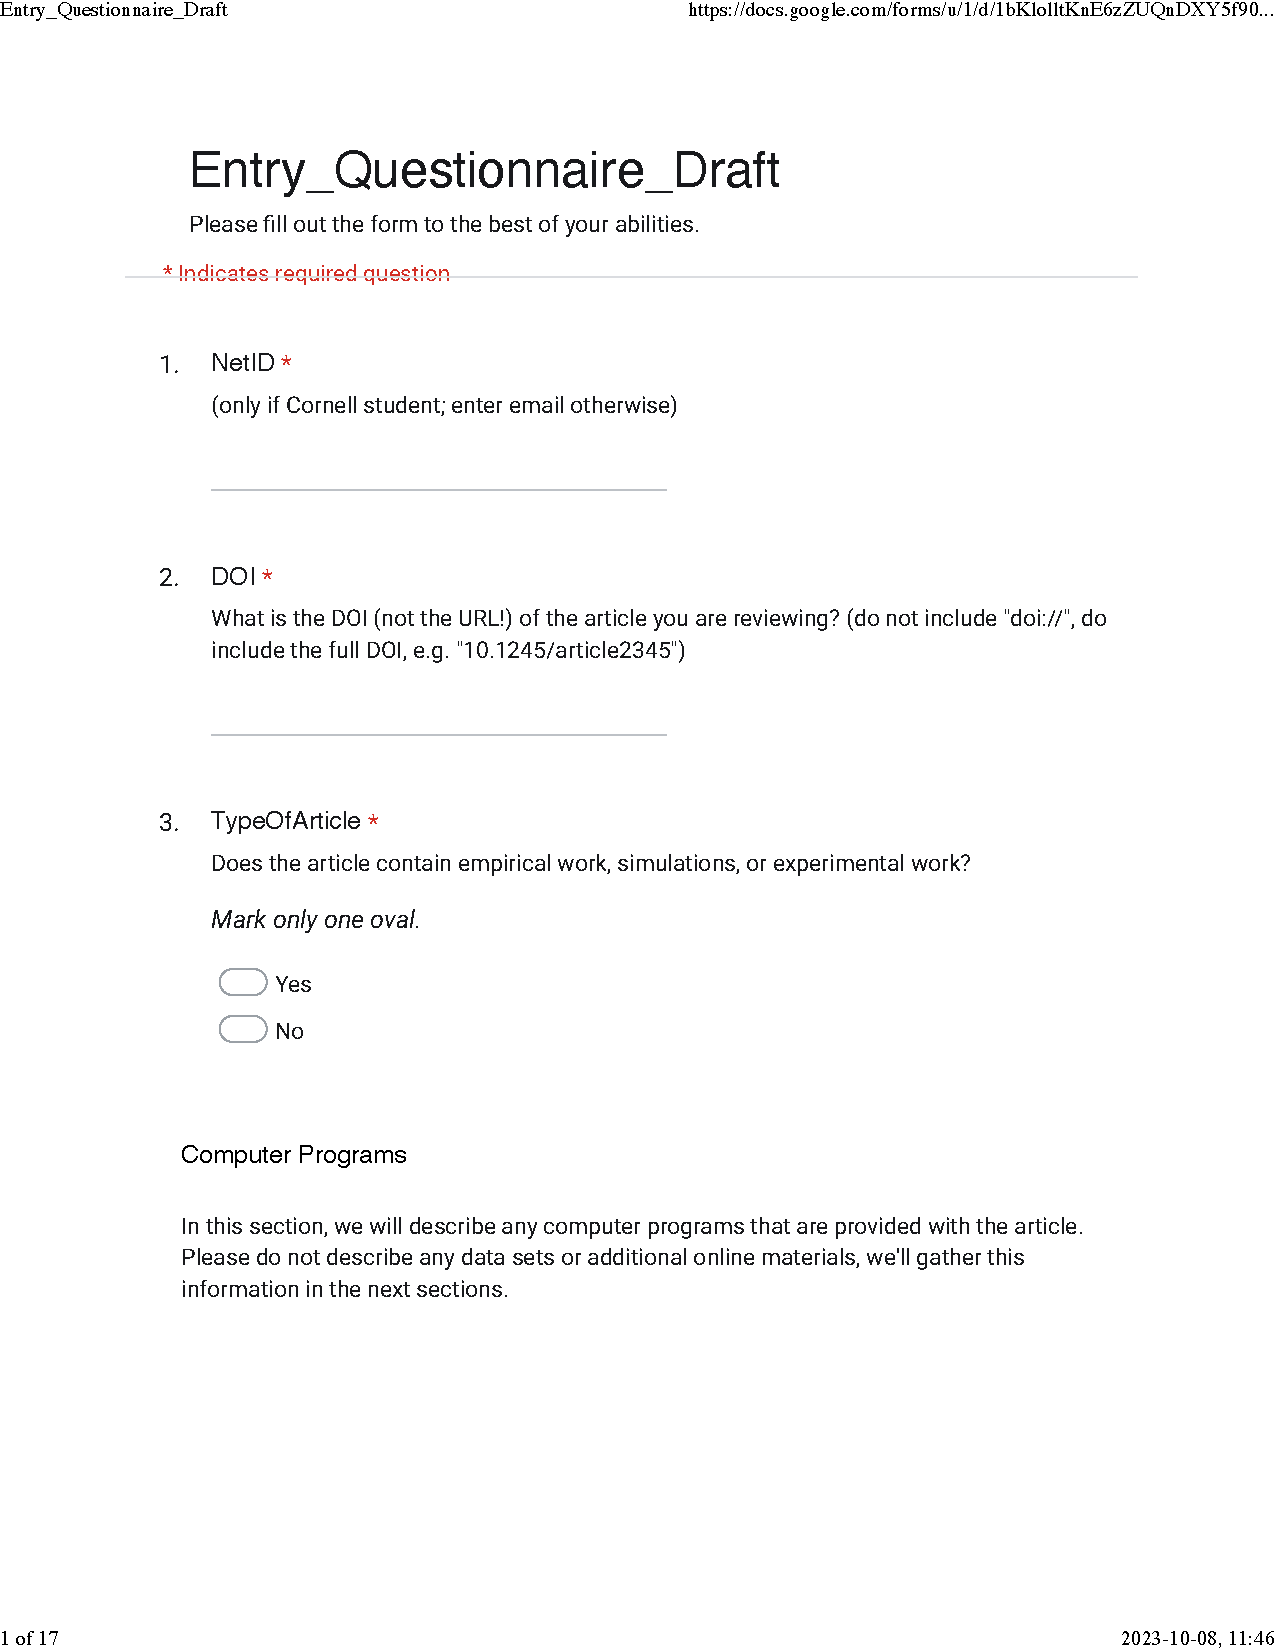
\includepdf[pages=1,scale=.8,pagecommand=\section{Assessment Questionnaire}\label{app:assessment_form}]{./includes/Entry_Questionnaire.pdf}
\includepdf[pages=2-,scale=.8,pagecommand={}]{./includes/Entry_Questionnaire.pdf}

% Exit Q
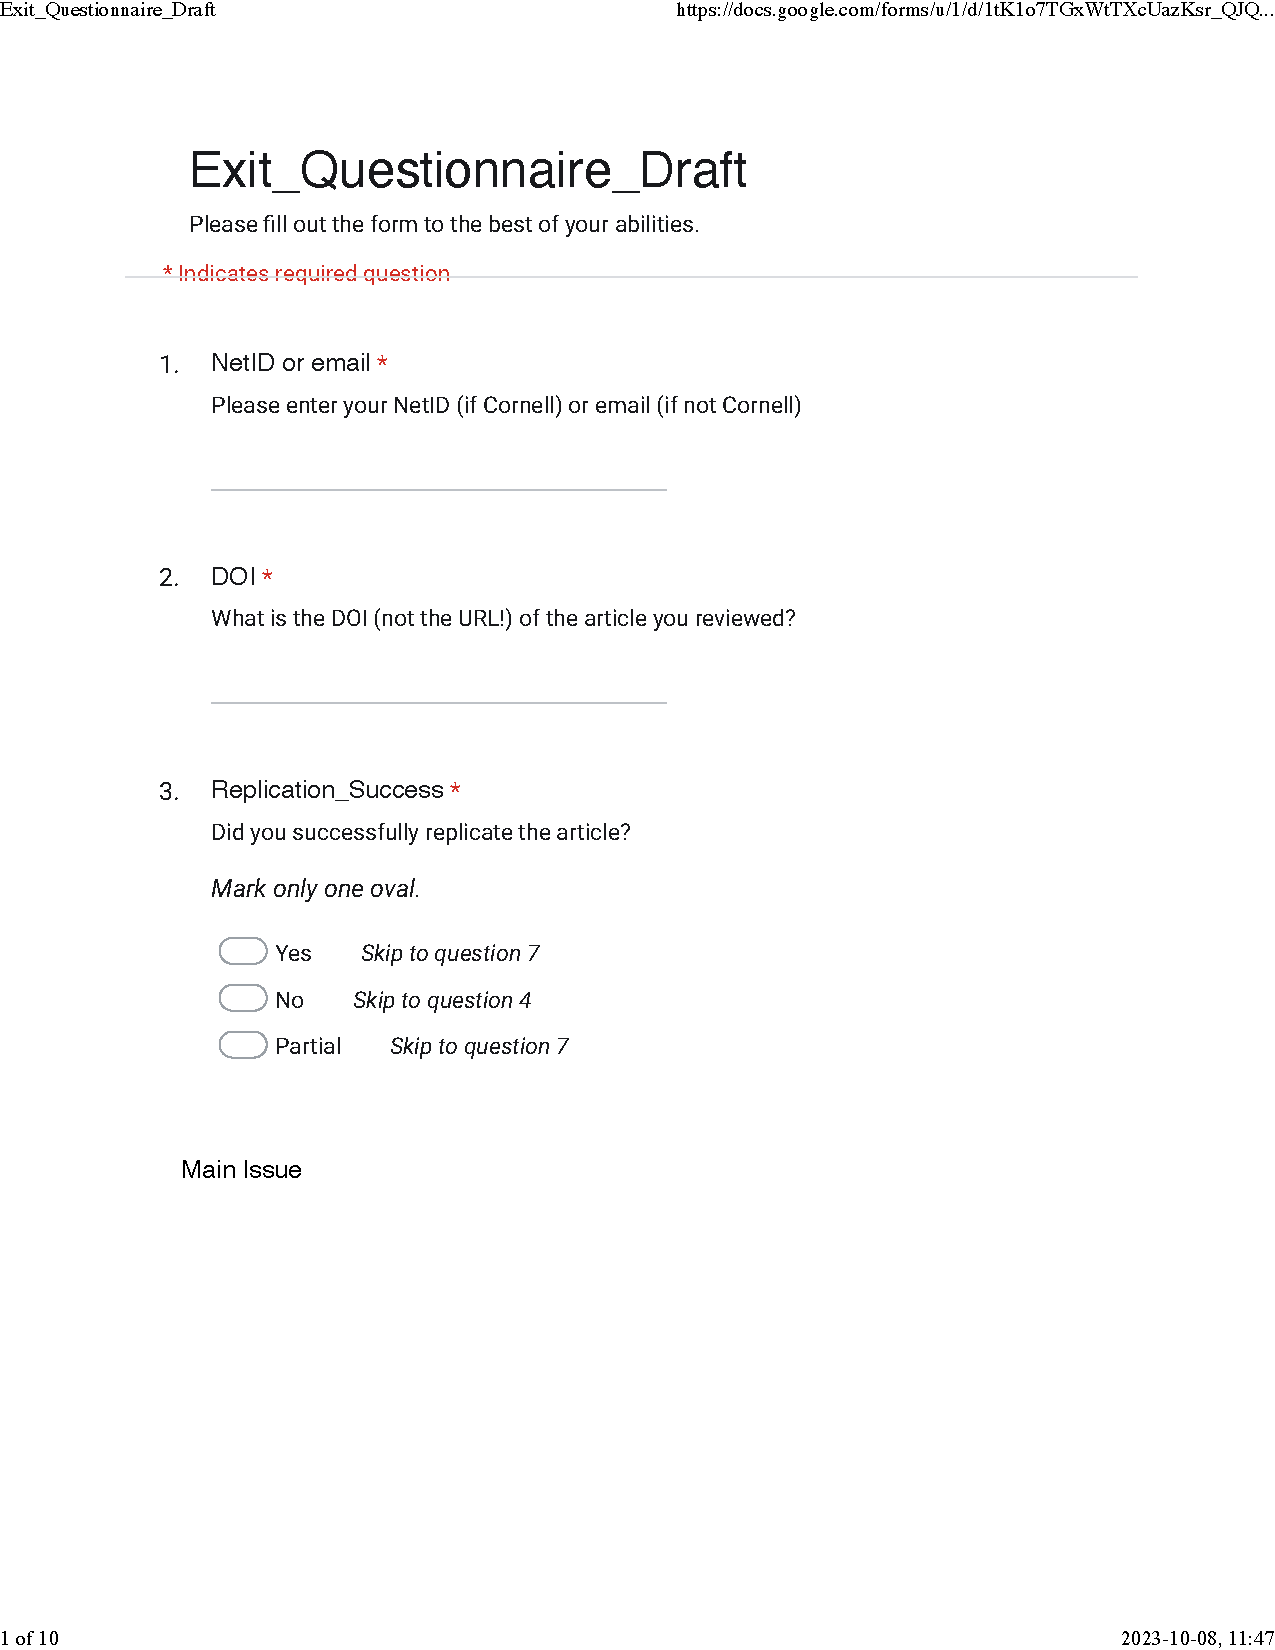
\includepdf[pages=1,scale=.8,pagecommand=\section{Exit Questionnaire}\label{app:exit_form}]{./includes/Exit_Questionnaire.pdf}
\includepdf[pages=2-,scale=.8,pagecommand={}]{./includes/Exit_Questionnaire.pdf}

\section{Replication Team}
The following members of the Replication Lab provided valuable assistance:

% first,initial,last,year
\csvreader[/csv/head=true,%
/csv/head to column names=true,%
/csv/late after line={,},%
/csv/late after last line=.,%
]%
{includes/Replication_Students_Historically.csv}{}{ \first \xspace \initial \xspace \last }

\newpage
\section{Acronyms Used}
%TCIDATA{Version=5.00.0.2570}
%TCIDATA{LaTeXparent=0,0,sw-edit.tex}

% $Id: acronyms.tex 1735 2017-06-23 15:47:39Z lv39 $
% $URL: https://forge.cornell.edu/svn/repos/ldi-replication/LaTeX/text/acronyms.tex $
%
% Define acronyms to be used in the text here. See
% http://www.mackichan.com/index.html?techtalk/456.htm~mainFrame for usage in
% Scientific workplace context

\begin{acronym}
\acro{ACS}{American Community Survey}
\acro{AEA}{American Economic Association}
\acro{AEJ:AE}{American Economic Journal: Applied Economics}
\acro{AEJ:Mac}{American Economic Journal: Macroeconomics}
\acro{AEJ:Mic}{American Economic Journal: Microeconomics}
\acro{AEJ:EP}{American Economic Journal: Economic Policy}
\acro{AER}{American Economic Review}
\acro{AJPS}{American Journal of Politial Science}
\acro{AHEAD}{Study of Assets and Health Dynamics Amongst the Oldest Old}
\acro{API}{application programming interface}
\acro{ASCII}{American Standard Code for Information  Interchange} %, typically used to denote raw text files in PC or Unix environments
\acro{ASM}{Annual Survey of Manufacturers}
\acro{BDS}{Business Dynamics Statistics}
\acro{BED}{Business Employment Dynamics}
\acro{BES}{Business Expenditure Survey}
\acro{BLS}{Bureau of Labor Statistics}
\acro{BRB}{Business Register Bridge}
\acro{BR}{Business Register}
\acro{CAC}{Cornell Center for Advanced Computing}
\acro{CBP}{County Business Patterns}
\acro{CBSA}{Core-Based Statistical Area}
\acro{CER}{Covered Earnings Records}
\acro{CES}{Center for Economic Studies}
\acro{CEW}{Covered Employment and Wages}%. Employment statistics program run by BLS in  conjunction with all states, also known as ES-202. Generally, when used  in this document, refers to public-use tabulations from the CEW, as  opposed to the confidential microdata received directly from the states.
\acro{CISER}{Cornell Institute for Social and Economic Research}
\acro{CIT}{Cornell Information Technologies}
\acro{CODA}{Children of Depression}
\acro{CPI}{Consumer Price Index}
\acro{CPI-U}{Consumer Price Index (All Urban Consumers)}
\acro{CPR}{Composite Person Record}
\acro{CPS}{Current Population Survey}
\acro{CRADC}{Cornell Restricted Access Data Center}
\acro{CTC}{Cornell Theory Center}
\acro{DCC}{Data Confidentiality Committee}
\acro{DOI}{Digital Object Identifier}
\acro{DER}{Detailed Earnings Record}
\acro{DRB}{Disclosure Review Board}
\acro{DWS}{Displaced Worker Supplement}
\acro{EJ}{Economic Journal}
\acro{ECF}{Employer Characteristics  File}
\acro{EHF}{Employment History Files}
%\acro{EIN}{\acroextra{(federal) }Employer Identification Number}
\acro{ERR}{Excess Reallocation Rate}
%\acro{ES-202}{ES-202\acroextra{. An older name for the \ac{QCEW} program}}
\acro{FHFA}{Federal Housing Finance Agency}
%\acro{FIPS}{Federal information processing standards codes\acroextra{\ issued     by \ac{NIST}}}
\acro{FSRDC}{Federal Statistical Research Data Center}
%\acro{FTI}{Federal Tax Information\acroextra{, typically covered under     Title 26, U.S.C.}}
\acro{GAL}{Geocoded Address List}
\acro{GIS}{Geographic Information System}
\acro{HPI}{House Price Index}
\acro{HRS}{Health and Retirement Study}
\acro{IAB}{Institute for Employment Research}
\acro{ICF}{Individual Characteristics File}
\acro{IRB}{Institutional Review Board}
\acro{IRS}{Internal Revenue Service}
\acro{ISR}{Institute for Social Research}
\acro{JCR}{Job Creation Rate}
\acro{JDR}{Job Destruction Rate}
\acro{JOLTS}{Job Openings and Labor Turnover Survey}
\acro{JASA}{Journal of the American Statistical Association}
\acro{JMCB}{Journal of Money, Credit and Banking}
\acro{JPE}{Journal of Political Economy}
\acro{JEEA}{Journal of the European Economic Association}
\acro{JRR}{Job Reallocation Rate}
\acro{LAUS}{Local Area Unemployment Statistics}
\acro{LBD}{Longitudinal Business Database}
%\acro{LDB}{\ac{BLS}'s Longitudinal Business Database}
\acro{LED}{Local Employment Dynamics}
\acro{LEHD}{Longitudinal Employer-Household Dynamics}
\acro{LMI}{Labor Market Information}
\acro{MBR}{Master Beneficiary Record}
\acro{MEF}{Master Earnings File}
\acro{MER}{Master Earnings Record}
\acro{MLS}{Mass Layoff Statistics}
\acro{MMS}{Methodology, Measurement, and Statistics}
\acro{MN}{Minnesota}
\acro{MSA}{Metropolitan Statistical Area}
\acro{MSD}{Metropolitan Statistical Division}
\acro{MWR}{Multiple Worksite Report}
\acro{NAICS}{North American Industry Coding System}
\acro{NECTA}{New England  City and Town Area}
\acro{NIA}{National Institute on Aging}
\acro{NIST}{National Institute of Standards and Technology}
\acro{NLSY}{National Longitudinal Study of Youth}
\acro{NSF}{National Science Foundation}
\acro{NSTA}{NAICS SIC Treatment of Auxiliaries}
\acro{OS}{operating system}
\acro{OTM}{OnTheMap}
\acro{PCF}{Person Characteristics File}
\acro{PHF}{Person History File}
\acro{PIK}{Protected Identity Key}
\acro{PSID}{Panel Study of Income Dynamics}
%\acro{QCEW}{Quarterly Census of Employment and Wages\acroextra{, managed by   the \acf{BLS}}}
\acro{QJE}{Quarterly Journal of Economics}
\acro{QWI}{Quarterly Workforce Indicators}
\acro{RDA}{Restricted Data Application}
\acro{RDC}{Research Data Center}
\acro{ReStat}{Review of Economics and Statistics}
\acro{RUN}{Reporting unit number}
%\acro{SEIN}{State employer identification number\acroextra{. It is     constructed from the state \ac{FIPS} code and the UI account     number. The BLS refers to the UI account number in combination with the     reporting unit number as SESA-ID}}
\acro{SEINUNIT}{SEIN reporting unit}
\acro{SEPB}{Summary of Earnings and Projected Benefits} % confidential SSA                                % file
%\acro{SESA-ID}{State Employment Security Agency ID\acroextra{. The UI     account number in combination with the Reporting Unit Number is treated   as a unique establishment identifier.}}
\acro{SESA}{State Employment Security Agency}
\acro{SIC}{Standard Industry Classification}
\acro{SIPP}{Survey of Income and Program Participation}
\acro{SLID}{Survey of Labour and Income Dynamics}
\acro{SPF}{Successor-Predecessor File}
\acro{SRMI}{Sequential Regression Multiple Imputation}
\acro{SSA}{Social Security Administration}
\acro{SSI}{Supplemental Security Income}
\acro{SSN}{Social Security Number}
\acro{SSR}{Supplemental Security Record}
%\acro{SynLBD}{Synthetic \ac{LBD}\acroextra{, a synthetic microdata file at the establishment level}}
\acro{U2W}{Unit-to-Worker Impute}
\acro{UI}{Unemployment Insurance}
\acro{URL}{Uniform Record Locator}
\acro{WB}{War Babies}
\acro{WIA}{Workforce Investment Act}
\acro{WIB}{Workforce Investment Board}
\acro{WRR}{Worker Reallocation Rate}
\acro{WTS}{Windows Terminal Services}
\acro{VCS}{version control system}
% Usage in the later text:
%  \ac{acronym}         Expand and identify the acronym the first time; use
%                       only the acronym thereafter
%  \acf{acronym}        Use the full name of the acronym.
%  \acs{acronym}        Use the acronym, even before the first corresponding
%                       \ac command
%  \acl{acronym}        Expand the acronym without using the acronym itself.
\end{acronym}

%%% Local Variables:
%%% mode: latex
%%% TeX-master: "proposal"
%%% End:


\end{document}

